\documentclass[12pt, a4paper]{article}

\usepackage[utf8]{inputenc}
\usepackage{mathtools}
\usepackage{amssymb}
\usepackage{ntheorem}
\usepackage[framemethod=TikZ]{mdframed}
\usepackage{amsmath}
\usepackage[hidelinks]{hyperref}
\usepackage{cleveref}
\usepackage{fancyhdr}
\usepackage{lastpage}
\usepackage{geometry}
\usepackage{arydshln}
\usepackage{url}
\usepackage{setspace}
\usepackage[T1]{fontenc}
\usepackage{framed}
\usepackage{pifont}
\usepackage{physics}

\geometry{a4paper, left=2cm, right=2cm, bottom=2cm, top=2cm}

\pagestyle{fancy}
\fancyhead{}
\fancyhead[L]{\leftmark}
\fancyhead[R]{\rightmark}
\fancyfoot{}
\fancyfoot[C]{\thepage}
%\renewcommand{\headrulewidth}{0pt}
\renewcommand{\footrulewidth}{0pt}

\linespread{1.25}

\hypersetup{
	colorlinks = true,
	bookmarks = true,
	bookmarksnumbered = true,
	pdfborder = 001,
	linkcolor = blue
}

\theorembodyfont{\upshape}
\theoremseparator{.}
\newtheorem{thm}{Theorem}[subsection]
\newtheorem{df}{Definition}[subsection]
\newtheorem{eg}{Example}[subsection]
\newenvironment*{sol}{\indent\textit{Solution. }}{\hfill{$\square$}\par}
\newtheorem*{rmk}{\indent Remark}
\newenvironment*{prf}{\indent\textbf{\textit{Proof. }}}{\hfill $\blacksquare$\par}
\newtheorem*{ext}{\indent Extension}

\def\Z{{\mathbb{Z}}}
\def\R{{\mathbb{R}}}
\def\C{{\mathbb{C}}}
\def\Q{{\mathbb{Q}}}
\def\E{{\mathbb{E}}}
\def\T{{\textbf{\emph{T}}}}
\def\d{{\mathrm{d}}}
\def\i{{\mathrm{i}}}
\def\RE{{\mathrm{Re}}}
\def\IM{{\mathrm{Im}}}
\def\Arg{{\mathrm{Arg}}}
\def\cis{\mathrm{cis}}
\def\rref{\mathrm{rref}}
\def\Span{\mathrm{Span}}
\def\Ker{\mathrm{Ker}}
\def\rank{\mathrm{rank}}
\def\nullity{\mathrm{nullity}}
\def\Proj{\mathrm{Proj}}
\def\Ref{\mathrm{Ref}}
\def\qed{\rightline{$\blacksquare$}}
\def\ddx{\frac{\d}{\d x}}
\def\dydx{\frac{\d y}{\d x}}
\def\dx{\d x}
\def\vecx{\vec{x}}
\def\vecy{\vec{y}}
\def\vecv{\vec{v}}
\def\vecw{\vec{w}}
\def\vecu{\vec{u}}
\def\veca{\vec{a}}
\def\vecb{\vec{b}}
\def\vece{\vec{e}}
\def\matrixA{\textbf{\emph{A}}}
\def\matrixB{\textbf{\emph{B}}}
\def\matrixD{\textbf{\emph{D}}}
\def\matrixI{\textbf{\emph{I}}}
\def\matrixM{\textbf{\emph{M}}}
\def\matrixN{\textbf{\emph{N}}}
\def\matrixS{\textbf{\emph{S}}}
\def\matrixP{\textbf{\emph{P}}}
\def\matrixU{\textbf{\emph{U}}}
\def\DNE{\mathrm{D.N.E.}}
\def\LI{\mathrm{L.I.}}

\title{Johns Hopkins University\\\textbf{AS.110.201 Linear Algebra}\\Learning Notes}
\author{Jiuru Lyu}
\date{\today}

\begin{document}

\maketitle

\tableofcontents

\newpage
\section*{Preface}
These are my personal notes for Johns Hopkins University AS.110.201 Linear Algebra course. I studied this course via Summer @ Hopkins in the summer of 2021. 

As no prerequisite is required (only pre-calculus, basic algebra, and some simple knowledge from Calculus I), this course focuses on matrices. It includes systems of linear equations, basics of matrices, spaces and dimensions, determinants, eigenvalues, and singular value decomposition. The textbook used for this course is \textit{Linear Algebra with Applications, 5th Edition} by Otto Bretscher. Another textbook by Gilbert Strang is also recommended: \textit{Introduction to Linear Algebra, 5th Edition}. 

Throughout this personal note, I use different formats to differentiate different contents, including definitions, theorems, proofs, examples, extensions, and remarks. To be more specific: 
\begin{df}[Terminology]
    This is a \textbf{definition}.	
\end{df}
\begin{thm}[Theorem Name]
    This is a \textbf{theorem}.	
\end{thm}
\begin{eg}
    This is  an \textbf{example}. 
\end{eg}

\begin{sol}
    This is the \textit{answer} part of an \textbf{example}. 
\end{sol}
\begin{rmk}
	This is a \textbf{remark} of a definition, theorem, example, or proof. 
\end{rmk}

\begin{prf}
	This is a \textbf{proof} of a theorem. 
\end{prf}
\begin{ext}
	This is a \textbf{extension} of a theorem, proof, or example. 	
\end{ext}

To better ace this course, it is recommended to do more questions than provided as examples under each section. Although each example is distinctive and representative, more questions and practice is still needed to deepen the understanding of this course. More than doing examples, using visualization tools to visualize some problems or concepts is also helpful in understanding the contents better. Videos made by \textbf{3Blue1Brown} are also recommended as a supplementary source of learning. 

Even though I put efforts into making as few flaws as possible when encoding these learning notes, some errors may still exist in this note. If you find any, please contact me via email: \url{lvjiuru@hotmail.com}. 

I hope you will find my notes helpful when learning Linear Algebra, a fundamental course for other Math and Computer Science courses. 

\rightline{Cheers,}
\rightline{Jiuru Lyu}

\newpage
\section{Systems of Linear Equations}
\subsection{Solving Systems of Linear Equations}

\begin{df}[Linear Equations]
An equation in the unknowns $x$, $y$, $z$, ... is called \textbf{linear} if both sides of the equation are a sum of multiples of $x$, $y$, $z$, ..., plus an optional constant. 
\end{df}
\begin{eg}
Linear equations and nonlinear equations\par
\begin{center}
$\left\{\begin{aligned}3x+4y&=2z\\-x-z&=100\end{aligned}\right.$ are linear equations,  but $\left\{\begin{aligned}3x+yz&=3\\\sin x-\cos y&=2\end{aligned}\right.$ are not.
\end{center}
\end{eg}

\begin{df}[System of Linear Equations]
A \textbf{system} of linear equations is a collection of several linear equations.
\end{df}

\begin{df}[Solution of a System]
A \textbf{solution} of a system of equations is a list of numbers $x$, $y$, $z$, ... that make all of the equations true simultaneously.
\end{df}

\begin{df}[Solution Set of a System]
The \textbf{solution set} of a system of equations is the collection of all solutions.
\end{df}

\begin{df}[Solving a System]
\textbf{Solving} the system means finding all solutions with formulas involving some number of parameters.
\end{df}

\begin{df}[Consistency and Inconsistency of a System]
A system of equations is called \textbf{inconsistent} if it has no solutions. It is called \textbf{consistent} otherwise. 
\end{df}

\begin{eg}
An inconsistent system: \par

\begin{center} $\left\{\begin{aligned}x+2y&=3\\x+2y&=-3\end{aligned}\right.$ has no solutions (the solution set is \textit{empty}).
\end{center}
Thus, the system of equations is \textbf{inconsistent}.
\end{eg}

\begin{rmk}
A solution of equations in $n$ variables is a list of $n$ numbers.
\end{rmk}

\begin{rmk}
We use $\R$ to denote the set of all real numbers.
\end{rmk}

\begin{df}[$\R^n$]
Let $n$ be a positive whole number. We define
$$\R^n=\text{all ordered }n\text{-tuples of real numbers }(x_1,\ x_2,\ x_3,\ ...,\ x_n)$$
An $n$-tuple of real number is called a \textbf{point} of $\R^n$
\end{df}
\begin{eg}
Examples of $\R^n$
\begin{enumerate}
\item $\left[0, \dfrac{3}{2},-\pi\right]$ and $(1, -2, 3)$ are points of $\R^3$
\item When $n=1$, $\R^1=\R$. Geometrically, this is the number line.
\item When $n=2$, $\R^2$. It becomes the $xy$-plane. 
\item When $n=3$, $\R^3$. It is the \textit{space} we live in. 
\end{enumerate}
\end{eg}


\begin{df}[Line]
A \textbf{line} is a ray that is \textit{straight} and \textit{infinite} in both directions.
\end{df}
\begin{df}[Plane]
A \textbf{plane} is a flat sheet that is infinite in all directions.
\end{df}
\begin{thm}
Generally, a single linear equation in $n$ variables defines an $(n-1)$-plane in $n$-space. 
\end{thm}

\begin{eg}
Examples of Lines and Planes. \par
\begin{enumerate}
\item \textbf{Lines}. For $x+y=1$ (implicit equation), the \textbf{parametric form} is $$(x,y)=(t, 1-t)\ \text{for any } t \in \R$$
We call $t$ a \textbf{parameter} in this case.
\item For a system of two linear equations (as implicit equations in $\R^3$) $$\left\{\begin{aligned}x+y+z&=1\\x-z&=0\end{aligned}\right., $$ the parametric form would be $$(x,y,z)=(t,1-2t,t)$$
\item \textbf{Planes}. For $x+y+z=1$ (implicit equation), the \textbf{parametric form} is $$(x,y,z)=(1-t-w,t,w) \text{ for any } t,w \in \mathbb{R}$$
\end{enumerate}
\end{eg}

\begin{thm}[Elementary Operations] Since elementary operations are reversible, the solution set doesn't change:
\begin{enumerate}
\item Switch the order of the equation;
\item Scale the equation by a scale $c\neq 0$; (to reverse, divide equation by $c$)
\item Add a multiple of one equation to another. (to reverse, subtract)
\end{enumerate}
\end{thm}

\subsection{Row Reduction}
\begin{thm}[The Elimination Method] We can use the \textbf{elimination} method to combine the equations in various ways to eliminate as many variables as possible for each equation.
\begin{enumerate}
\item \textbf{Scaling}. We can multiply both sides of an equation by a nonzero number. 
\item \textbf{Replacement}. We can add a multiple of one equation to another, replacing the second equation with the result. 
\item \textbf{Swap}. We can swap two equations.
\end{enumerate}
\end{thm}

\begin{df}[Augmented Matrices and Row Operations]
\textbf{Augmented Matrix} refers to the vertical line, which we draw to remind ourselves where the equals sign belongs.
\end{df}

\begin{df}[Matrix]
A \textbf{matrix} is a grid of numbers without the vertical line. 
\end{df}

\begin{eg}
Augmented Matrix and Row Operations. \par
\begin{center}
$\left[\begin{array}{c:c}\begin{matrix}1&2&3\\2&-3&2\\3&1&-1\end{matrix}&\begin{matrix}6\\14\\-2\end{matrix}\end{array}\right]$ is an augmented matrix. 
\end{center}
The three ways of manipulating our equations become row operations:
\begin{enumerate}
\item \textbf{Scaling}. multiply all entries in a row by a nonzero number. 
$$\left[\begin{array}{c:c}\begin{matrix}1&2&3\\2&-3&2\\3&1&-1\end{matrix}&\begin{matrix}6\\14\\-2\end{matrix}\end{array}\right]\xrightarrow[]{R_1=R_1\times-3} \left[\begin{array}{c:c}\begin{matrix}-3&-6&-9\\2&-3&2\\3&1&-1\end{matrix}&\begin{matrix}-18\\14\\-2\end{matrix}\end{array}\right]$$
\begin{rmk}Here, the notation $R_1$ simply means "the first row."\end{rmk}
\item \textbf{Replacement}. add a multiple of one row to another, replacing the second row with the result. 
$$\left[\begin{array}{c:c}\begin{matrix}1&2&3\\2&-3&2\\3&1&-1\end{matrix}&\begin{matrix}6\\14\\-2\end{matrix}\end{array}\right]\xrightarrow[]{R_2=R_2-2\times R_1} \left[\begin{array}{c:c}\begin{matrix}1&2&3\\0&-7&-4\\3&1&-1\end{matrix}&\begin{matrix}6\\2\\-2\end{matrix}\end{array}\right]$$
\item \textbf{Swap}. Interchange two rows. 
$$\left[\begin{array}{c:c}\begin{matrix}1&2&3\\2&-3&2\\3&1&-1\end{matrix}&\begin{matrix}6\\14\\-2\end{matrix}\end{array}\right]\xrightarrow[]{R_1\leftrightarrow R_3} \left[\begin{array}{c:c}\begin{matrix}-3&-6&-9\\2&-3&2\\3&1&-1\end{matrix}&\begin{matrix}-18\\14\\-2\end{matrix}\end{array}\right]$$
\end{enumerate}
\end{eg}

\begin{df}[Row equivalent]
Two matrices are called \textbf{row equivalent} if one can be obtained from the other by doing some number of row operations. 
\end{df}

\begin{df}[Row Echelon Form (\emph{ref}) of Matrix]
A matrix is in \textbf{row echelon form} if: 
\begin{enumerate}
\item All zero rows are at the bottom.
\item The first nonzero entry of a row is to the \textit{right} of the first nonzero entry of the row above. 
\item Below the first nonzero entry of a row, all entries are zero.
\end{enumerate}
\end{df}

\begin{eg} 
General \emph{ref} of matrices. 
$$\left[\begin{array}{c:c}\begin{matrix}\textcolor{red}{a}&b&b&b\\0&\textcolor{red}{a}&b&b\\0&0&0&\textcolor{red}{a}\\0&0&0&0\end{matrix}&\begin{matrix}b\\b\\b\\0\end{matrix}\end{array}\right], $$

where $b=$ is any number, and $\textcolor{red}{a}=$ is any nonzero number.
\end{eg}
\begin{df}[Pivot]
A \textbf{\textit{pivot}} is the first nonzero entry of a row of a matrix in row echelon form.
\end{df}

\begin{df}[Reduced Row Echelon Form (\emph{rref}) of a Matrix]
A matrix is in \textbf{reduced row echelon form} if it is in row echelon form, and in addition:
\begin{enumerate}
\item[4.] Each pivot is equal to 1. 
\item[5.] Each pivot is the only nonzero entry in its column.
\end{enumerate}
\end{df}

\begin{eg}
Genderal \emph{rref} of matrices
$$\left[\begin{array}{c:c}\begin{matrix}\textcolor{red}{1}&0&b&0\\0&\textcolor{red}{1}&b&0\\0&0&0&\textcolor{red}{1}\\0&0&0&0\end{matrix}&\begin{matrix}b\\b\\b\\0\end{matrix}\end{array}\right], $$

where $b=$ is any number, $\textcolor{red}{1}=$ pivot
$$\left[\begin{array}{c:c}\begin{matrix}1&0&0\\0&1&0\\0&0&1\end{matrix}&\begin{matrix}1\\-2\\3\end{matrix}\end{array}\right]\xrightarrow[]{becomes} \left\{\begin{aligned}x&=1\\y&=-2\\z&=3\end{aligned}\right.$$
\end{eg}

\begin{thm}
Every matrix is row equivalent to one and only one matrix in reduced row echelon form.

\textbf{\textit{Row reduction}} or \textbf{\textit{Gaussian elimination}} demonstrates that every matrix is row equivalent to a least one matrix in reduced row echelon form. 
\begin{enumerate}
\item Swap the 1$^\text{st}$ row with a lower one, so a leftmost nonzero entry is in the 1st row (if necessary).
\item Scale the 1$^\text{st}$ row so that its first nonzero entry equals 1.
\item Use row replacement, so all entries below this 1 are 0.
\item Swap the 2$^\text{nd}$ row with a lower one so that the leftmost nonzero entry is in the 2nd row.
\item Scale the 2$^\text{nd}$ row so that its first nonzero entry equals 1.
\item Use row replacement, so all entries below this 1 are 0.
\item Swap the 3$^\text{rd}$ row with a lower one so that the leftmost nonzero entry is in the 3rd row.
etc.
\item Use row replacement to clear all entries above the pivots, starting with the last pivot.
\end{enumerate}
\end{thm}

\begin{df}[Pivot Position]
A \textbf{pivot position} of a matrix is an entry that is a pivot of a row echelon form of that matrix.
\end{df}
\begin{df}[Pivot Column]
A \textbf{pivot column} of a matrix is a column that contains a pivot position.
\end{df}

\begin{thm}[The Row Echelon Form of an Inconsistent System] An augmented matrix corresponds to an inconsistent system of equations if and only if (\emph{iff}) the last column (i.e., the augmented column) is a pivot column.
\end{thm}

\subsection{Parametric Form}
\begin{df}[Free Variable]
Consider a consistent system of equations in the variables $x_1$, $x_2$,..., $x_n$. Let $A$ be a row echelon form of the augmented matrix for this system. We say that $x_i$ is a \textbf{free variable} if its corresponding column in $A$ is not a pivot column.
\end{df}

\begin{eg} Example of free variables.

In the matrix $\left[\begin{array}{c:c}\begin{matrix}1&0&\textcolor{red}{5}\\0&1&\textcolor{red}{2}\end{matrix}&
\begin{matrix}1\\-2\end{matrix}\end{array}\right]$, the variable $\textcolor{red}{z}$ is the free variable.
\end{eg}

\begin{df}[Implicit Equations]
The line is defined implicitly as the simultaneous solutions to those equations.
\end{df}

\begin{df}[Parameterized Equations]
A \textbf{parameterized equation} is an expression that produces all points of the line in terms of one parameter. 
\end{df}

\begin{eg}
Example of implicit equations.
$\left\{\begin{aligned}2x+y+12z&=1\\x+2y+9z&=-1\end{aligned}\right.$ is an example of implicit equations in $\R^3$. $\left\{\begin{aligned}x&=1-5z\\y&=1-2z\end{aligned}\right.$ can be written as $(x,y,z,)=(1-5z, 1-2z,z),\ z \in \R$, which is a parameterized equation.
\begin{rmk} One should think of a system of equations as an implicit equation for its solution set and of the parametric form as the parameterized equation for the same set. The parametric form is much more explicit: it gives a concrete recipe for producing all solutions.
\end{rmk}
\end{eg}
\begin{thm}[Number of Solutions]
Systems of equations can have different numbers of solutions. 
\begin{enumerate}
\item \textbf{The last column is a pivot column}. In this case, the system is inconsistent. It has zero solutions. 
\item \textbf{Every column except the last column is a pivot column}. The system has a unique solution.
\item \textbf{The last column is not a pivot column, and some other column is not a pivot column either}. The system has many solutions corresponding to the infinite possible values of the free variables.
\end{enumerate}
\end{thm}

\begin{eg} 
Systems with different numbers of solutions. 
\begin{enumerate}
\item  $\left[\begin{array}{c:c}\begin{matrix}1&0\\0&1\\0&0\end{matrix} &\begin{matrix}\textcolor{red}{0}\\\textcolor{red}{0}\\\textcolor{red}{1}\end{matrix}\end{array}\right]$ comes form a linear system with no solutions.
\item For the matrix $\left[\begin{array}{c:c}\begin{matrix}1&0&0\\0&1&0\\0&0&1\end{matrix}&\begin{matrix}a\\b\\c\end{matrix}\end{array}\right]$, it has a unique solution $(x,y,z)=(a,b,c)$
\end{enumerate}
\end{eg}


\newpage
\section{Vector Equations and Linear Transformations}
\subsection{Vectors}

\begin{df}[Vector]
A \textbf{vector} is an array of n numbers: $$\vec{x} (\text{or }\bold{x})=\begin{bmatrix}x_1\\x_2\\\vdots\\x_n\end{bmatrix}$$
\end{df}

\begin{df}[$\R^n$]
A set of all vectors of height in n is denoted in $\R^n$.
\end{df}

\begin{thm}[Vector Addition]
$$\begin{bmatrix}a\\b\\c\end{bmatrix}+\begin{bmatrix}x\\y\\z\end{bmatrix}=\begin{bmatrix}a+x\\b+y\\c+z\end{bmatrix}$$
\end{thm}
\begin{thm}[Scalar multiplication]
$$\textcolor{red}{c}\times\begin{bmatrix}x\\y\\z\\ \end{bmatrix}=\begin{bmatrix}\textcolor{red}{c}\times x\\\textcolor{red}{c}\times y\\\textcolor{red}{c}\times z\end{bmatrix}$$
\end{thm}

\begin{eg}
The vector $\vec{v}=\begin{bmatrix}1\\2\end{bmatrix}$ is shown on a $xy$-plane as the following: 
\begin{figure}[H]
\centering
\includegraphics[width=0.25\textwidth]{vector1.png}
\end{figure}
\begin{enumerate}
\item The vector addition of $\begin{bmatrix}1\\2\end{bmatrix}+\begin{bmatrix}2\\3\end{bmatrix}=\begin{bmatrix}3\\5\end{bmatrix}$ will be: 
\begin{figure}[H]
\centering
\includegraphics[width=0.5\textwidth]{vector addition.png} 
\end{figure}
\item The vector scalar multiplication of $3\begin{bmatrix}1\\2\end{bmatrix}$ will be: \begin{figure}[H] 
\centering 
\includegraphics[width=0.25\textwidth]{scalar multiplication.png} 
\end{figure}
\end{enumerate}
\end{eg}

\begin{ext}The Parallelogram Law for Vector Addition.\end{ext}

\begin{ext}Vector Subtraction.\end{ext}

\begin{df}[Linear Combinations]
Let $c_1,c_2,...,c_k$ be scalars, and let $v_1,v_2,...,v_k$ be vectors in $\R^2$. The vector in $\R^2$ $$c_1v_1+c_2v_2+...+c_kv_k$$ is called a \textbf{linear combination} of the vectors $v_1,v_2,...,v_k$ with \textbf{weights} or \textbf{coefficients} $c_1,c_2,...,c_k$.
\end{df}

\subsection{Vector Equations}
\begin{df}[Vector Equation]
A \textbf{vector equation} is an equation involving a linear combination of vectors with possibly unknown coefficients.
\end{df}

\begin{eg}
Asking whether or not a vector equation has a solution is the same as asking if a given vector is a linear combination of some other given vector. 

The equation 
$$x\begin{bmatrix}1\\2\\6\end{bmatrix}+y\begin{bmatrix}-1\\-2\\-6\end{bmatrix}=\begin{bmatrix}8\\16\\3\end{bmatrix}$$ 
is asking if the vector $\begin{bmatrix}8\\16\\3\end{bmatrix}$ is a linear combination of the vectors $\begin{bmatrix}1\\2\\6\end{bmatrix}$ and $\begin{bmatrix}-1\\-2\\-6\end{bmatrix}$. 

The equation can be simplified to 
$$\begin{bmatrix}x-y\\2x-2y\\6x-y\end{bmatrix}=\begin{bmatrix}8\\16\\3\end{bmatrix} \ \text{or}\ \left\{\begin{aligned}x-y&=8\\2x-2y&=16\\6x-y&=3\end{aligned}\right.$$.\\Then, one can use augmented matrix to solve it.
\end{eg}
\begin{rmk}Three equivalent ways of thinking about a linear system: 
\begin{enumerate}
\item A system of equations
\item An augmented matrix
\item A vector equation
\end{enumerate}
\end{rmk}

\begin{thm}
A new way to consider linear systems.

Suppose the LHS of a linear system is something we can plug a vector into to produce a list of numbers, and the RHS of a linear system shows the solution out as a vector. 

Thus, The LHS of a system is a function $\textbf{\textit{T}}:\ \R^m \rightarrow \R^n$, where $m$ is the number of variables and $n$ is the number of equations. 

To solve the system, we want to find all vectors that will map to a particular group. We can record the function associated with the LHS of a system as a matrix. 
\end{thm}

\begin{eg}
Example of converting linear systems to matrix equations. 

The linear system $$\left\{\begin{aligned}7x_1+3x_2+4x_3&=25\\2x_1+0x_2+x_3&=5\end{aligned}\right.$$ 
can be recorded as
$$\begin{bmatrix}7&3&4\\2&0&1\end{bmatrix}\begin{bmatrix}x_1\\x_2\\x_3\\\end{bmatrix}=\begin{bmatrix}25\\5\end{bmatrix}$$
\end{eg}

\begin{thm}
Multiplication of a vector by a matrix.
\begin{enumerate}
\item For each row of the matrix, multiply the entries of that row with the corresponding entries of the vector and then add.
\item The output vector is the final output. 
\end{enumerate}
\end{thm}

\begin{eg}
 
$$\begin{bmatrix}7&3&4\\2&0&1\end{bmatrix}\begin{bmatrix}1\\1\\1\\\end{bmatrix}=\begin{bmatrix}7\times 1+3\times 1+4\times 1\\2\times 1+0\times 1+1\times 1\end{bmatrix}=\begin{bmatrix}14\\3\end{bmatrix}$$
\end{eg}

\subsection{Linear Transformation}
\begin{df}[Linear Transformation]
A \textbf{linear transformation} is a function $\T: \R^m\rightarrow\R^n$ so that:
\begin{enumerate}
\item $\T(\vec{x}+\vec{y})=\T(\vec{x})+\T(\vec{y})$
\item $\T(c\times \vec{x})=c\times\T(\vec{x})$
\end{enumerate}
$$\forall \vec{x},\vec{y}\in \R^m\text{, and }c\in\R$$
\end{df}

\begin{df}[Standard Basis Vectors]
The vectors $\vece_1,\vece_2,...,\vece_n \in \R^m$ defined by 
$$\vece_i=\begin{bmatrix}0\\\vdots\\1\\\vdots\\0\end{bmatrix} \rightarrow \ \text{the }i\text{-th entry}$$ are called the \textbf{standard basis vectors}.
\end{df}

\begin{thm}
Let $\T: \R^m\rightarrow\R^n$ be a linear transformation, and $$\matrixA=\begin{bmatrix}\vdots&\vdots&\cdots&\vdots\\\T \vece_1&\T \vece_2&\cdots&\T \vece_n\\\vdots&\vdots&\cdots&\vdots\end{bmatrix}$$ Then, $\T\vecx=\matrixA\vecx$ for all vectors $\vecx$
\end{thm}

\begin{prf}
Assume $\vec{x}=\begin{bmatrix}x_1\\\vdots\\x_n\end{bmatrix}$, then $\vec{x}=x_1\vece_1+x_2\vece_2+...+x_n\vece_n$.\\Thus, $$\T\vec{x}=x_1\boldsymbol{T}\vece_1+x_2\T \vece_2+...+x_n\T \vece_n= \begin{bmatrix}\vdots&\vdots&\cdots&\vdots\\\T{\vece_1}&\T{\vece_2}&\cdots&\T{\vece_n}\\\vdots&\vdots&\cdots&\vdots\end{bmatrix}\begin{bmatrix}x_1\\\vdots\\x_n\end{bmatrix}=\matrixA\vec{x}$$
\end{prf}

\begin{thm}
Given any sequence of elementary raw operations $s_1, s_2,...,s_k$ involving n-rows, there exists a matrix $\matrixB$ such that for all $\vec{v}\in\R^n$, $\matrixB\vec{v}$ equals that vector obtained by applying $s_1, s_2,...,s_k$ to $\vec{v}$.
\end{thm}

\begin{eg}
$$\begin{bmatrix}x\\y\end{bmatrix}\xrightarrow[]{\text{II}-\text{I}}\begin{bmatrix}x\\y-x\end{bmatrix}\xrightarrow[]{\text{I}-\text{II}}\begin{bmatrix}2x-y\\y-x\end{bmatrix}\begin{bmatrix}x\\y\end{bmatrix}=\begin{bmatrix}2&-1\\1&-1\end{bmatrix}\begin{bmatrix}x\\y
\end{bmatrix},$$

where $\begin{bmatrix}2&-1\\1&-1\end{bmatrix}$ is the matrix $\matrixB$
\end{eg}

\begin{df}[Geometric Definition of Linear Transformation]
We can also think of linear transformation from a geometric perspective. 

\begin{enumerate}
\item $\T: \R^m\rightarrow\R^n$ implies that the original parallelograms map to the transformed parallelograms
\item $\T(c\times \vec{x})=c\times\T(\vec{x})$ means that the original lines through the origin map to the transformed lines through the origin, and the original maps the ruling defined with fundamental unit $\vec{x}$ to ruling with unit $\T\vec{x}$
\item Rotation around the origin is a linear transformation. 
\item Reflection through a line through the origin is a linear transformation.
\item Translation is not a linear transformation.
\end{enumerate}
\end{df}

\begin{eg}
Fix $\theta \in [0, 2\pi )$. Consider the map $\text{Rot}_\theta: \R^2 \rightarrow\R^2$, which rotates a vector by angle $\theta$ around the origin counterclockwise. $\text{Rot}_\theta$ is a linear transformation. Find the matrix associated with this transformation.\\
\begin{sol}
Let $\vece_1=\begin{bmatrix}1\\0\end{bmatrix},\ \vece_2=\begin{bmatrix}0\\1\end{bmatrix}$. \\
The matrix of $\text{Rot}_\theta$ is 
$$\begin{bmatrix}|&|\\ \text{Rot}_{\theta}\vece_1& \text{Rot}_{\theta}\vece_2\\|&|\end{bmatrix}$$
\begin{enumerate}
\item If $\theta = \dfrac{\pi}{2}$, i.e. we rotate by 90° counterclockwise. The matrix for rotation is $$\begin{bmatrix}|&|\\ \text{Rot}_{\theta}\vece_1& \text{Rot}_{\theta}\vece_2\\|&|\end{bmatrix}=\begin{bmatrix}|&|\\ \vece_2& -\vece_2\\|&|\end{bmatrix}=\begin{bmatrix}0&-1\\1&0\end{bmatrix}$$
\item General case: 
$e_1=\begin{bmatrix}1\\0\end{bmatrix};e_2=\begin{bmatrix}0\\1\end{bmatrix}$. Thus, $$\text{Rot}_{\theta}\vece_1=\begin{bmatrix}\cos{\theta}\\\sin{\theta}\end{bmatrix};\text{Rot}_{\theta}\vece_2=\begin{bmatrix}0&-1\\1&0\end{bmatrix}\begin{bmatrix}\cos{\theta}\\\sin{\theta}\end{bmatrix}=\begin{bmatrix}-\sin{\theta}\\\cos{\theta}\end{bmatrix}.$$
$$\Longrightarrow\begin{bmatrix}|&|\\ \text{Rot}_{\theta}\vece_1& \text{Rot}_{\theta}\vece_2\\|&|\end{bmatrix}=\begin{bmatrix}\cos{\theta}&-\sin{\theta}\\\sin{\theta}&\cos{\theta}\end{bmatrix}$$
\begin{figure}[H] 
\centering 
\includegraphics[width=0.5\textwidth]{Rotation.png}
\end{figure}
\end{enumerate}
\end{sol}
\end{eg}

\begin{eg}
The map $\text{Ref}_L:\R^2\rightarrow\R^2$ is a linear transformation that reflects a vector over the line $L: y=2x$. Find the matrix for $\text{Ref}_L$.\\
\begin{sol}
Key idea: express $\vece_i=\vece_i^\parallel+\vece_i^\perp$, and $\text{Ref}(\vece_i)=\text{Ref}(\vece_i^\parallel)+\text{Ref}(\vece_i^\perp)$. \\
Choose $\begin{bmatrix}1\\2\end{bmatrix} \in L$, then every parallel vector is $c\begin{bmatrix}1\\2\end{bmatrix}$.\\
Rotate $\begin{bmatrix}1\\2\end{bmatrix}$ by 90°: $$\begin{bmatrix}0&-1\\1&0\end{bmatrix}\begin{bmatrix}1\\2\end{bmatrix}=\begin{bmatrix}-2\\1\end{bmatrix}, $$
then are perpendicular vector is $d\begin{bmatrix}-2\\1\end{bmatrix}$. \\
Take $\vece_1=\begin{bmatrix}1\\0\end{bmatrix}$ and $\vece_2=\begin{bmatrix}0\\1\end{bmatrix}$, then we get
$$\begin{cases}\begin{bmatrix}1\\0\end{bmatrix}&=c\begin{bmatrix}1\\2\end{bmatrix}+d\begin{bmatrix}-2\\1\end{bmatrix}\\\begin{bmatrix}0\\1\end{bmatrix}&=c^{'}\begin{bmatrix}1\\2\end{bmatrix}+d^{'}\begin{bmatrix}-2\\1\end{bmatrix}\end{cases}\Longrightarrow\begin{cases}c=\frac{1}{5}\\d=-\frac{2}{5}\\c^{'}=\frac{2}{5}\\d^{'}=\frac{1}{5}\end{cases}\Longrightarrow\begin{cases} e_1=\frac{1}{5}\begin{bmatrix}1\\2\end{bmatrix}-\frac{2}{5}\begin{bmatrix}-2\\1\end{bmatrix}\\e_2=\frac{2}{5}\begin{bmatrix}1\\2\end{bmatrix}+\frac{1}{5}\begin{bmatrix}-2\\1\end{bmatrix}\end{cases};$$
$$\xrightarrow{\ \ \ \ \ \ \ \ \text{Ref}_L\ \ \ \ \ \ \ \ }\begin{cases}\text{Ref}_L(\vece_1)=\frac{1}{5}\begin{bmatrix}1\\2\end{bmatrix}+\frac{2}{5}\begin{bmatrix}-2\\1\end{bmatrix}=\begin{bmatrix}^{-3}/_5\\^4/_5\end{bmatrix}\\\text{Ref}_L(\vece_2)=\frac{2}{5}\begin{bmatrix}1\\2\end{bmatrix}-\frac{1}{5}\begin{bmatrix}-2\\1\end{bmatrix}=\begin{bmatrix}^4/_5\\^3/_5\end{bmatrix}\end{cases}.$$
Thus, the matrix is 
$$\left[\begin{array}{cc}^{-3}/_{5}&^4/_{5}\\ ^{4}/_{5}&^{3}/_{5}\end{array}\right].$$
\end{sol}
\end{eg}

\newpage
\section{Matrices}
\subsection{Matrix Multiplication}
\begin{thm}[Procedure of Matrix Multiplication]
Matrix multiplication is very different from other formats of multiplication.
\begin{itemize}
	\item Input: a pair of matrices $\matrixA$ and $\matrixB$. \\
	*The number of rows of $\matrixA$ equals the number of columns of $\matrixB$.
	\item Output: The product $\matrixB\matrixA$
	\item Procedure: 
	\begin{enumerate}
		\item View $\matrixA$ as a list of its column vectors: 
		\[\matrixA=\begin{bmatrix}|& &|\\v_1&\cdots &v_n\\|& &|\end{bmatrix}\]
		\item Multiply each column by $\matrixB$: 
		\[\matrixB\matrixA =\begin{bmatrix}|& &|\\\matrixB v_1&\cdots &\matrixB v_n\\|& &|\end{bmatrix}\]
	\end{enumerate}
\end{itemize}	
\end{thm}

\begin{eg}
Examples of matrix multiplication.
\begin{enumerate}
	\item Let $\matrixA=\begin{bmatrix}1&2\\-1&1\end{bmatrix}$ and $\matrixB=\begin{bmatrix}1&2\\0&1\\3&5\end{bmatrix}$. Find $\matrixB\matrixA$.\\
	\begin{sol}\[\matrixB\matrixA=\begin{bmatrix}1&2\\0&1\\3&5\end{bmatrix}\begin{bmatrix}1&2\\-1&1\end{bmatrix}=\begin{bmatrix}1\times1+2\times(-1)&2\times1+2\times1\\1\times0+1\times(-1)&0\times2+1\times1\\3\times1+5\times(-1)&3\times1+5\times1\end{bmatrix}=\begin{bmatrix}-1&4\\-1&1\\-2&11\end{bmatrix}\]\end{sol}
	\item Let $\matrixA=\begin{bmatrix}1&2\\0&1\\3&5\end{bmatrix}$ and $\matrixB=\begin{bmatrix}1&2\\-1&1\end{bmatrix}$. Find $\matrixB\matrixA$.\\
	\begin{sol} Because 2 columns is not equal to three rows, the product does not exist. \end{sol}
	\item Let $\matrixA=\begin{bmatrix}1&2\\-1&1\end{bmatrix}$ and $\matrixB=\begin{bmatrix}1&0&3\\2&1&5\end{bmatrix}$. Find $\matrixA\matrixB$.\\
	\begin{sol}\[	\matrixA\matrixB=\begin{bmatrix}1&2\\-1&1\end{bmatrix}\begin{bmatrix}1&0&3\\2&1&5\end{bmatrix}=\begin{bmatrix}1\times1+2\times2&0\times1+2\times1&3\times1+2\times5\\-1\times1+2\times1&0\times(-1)+1\times1&3\times(-1)+5\times1\end{bmatrix}\\=\begin{bmatrix}5&2&13\\1&1&2\end{bmatrix}\]\end{sol}
\end{enumerate}	
\end{eg}

\begin{rmk}[Conceptualizing Matrix Multiplication]
There are many ways to understand matrix multiplication: 
\begin{enumerate}
	\item A matrix encodes a linear transformation: 
	\[ \matrixA: \R^m\longrightarrow\R^n\text{ is a }m\times n\text{ matrix.}\]
	\[ \matrixB: \R^n\longrightarrow\R^k\text{ is a }n\times k\text{ matrix.}\]
	We can compass these maps: 
	\begin{center}
	\tikzset{every picture/.style={line width=0.75pt}}  
	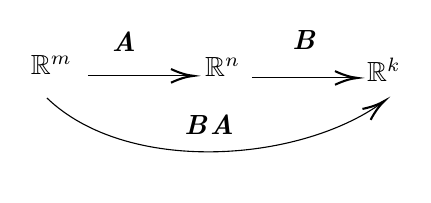
\begin{tikzpicture}[x=0.75pt,y=0.75pt,yscale=-1,xscale=1]
	\draw    (150.74,156.35) -- (199.74,156.35) ;
	\draw [shift={(201.74,156.35)}, rotate = 180] [color={rgb, 255:red, 0; green, 0; blue, 0 }  ][line width=0.75]    (10.93,-3.29) .. controls (6.95,-1.4) and (3.31,-0.3) .. (0,0) .. controls (3.31,0.3) and (6.95,1.4) .. (10.93,3.29)   ;
	\draw    (229.74,157.35) -- (278.74,157.35) ;
	\draw [shift={(280.74,157.35)}, rotate = 180] [color={rgb, 255:red, 0; green, 0; blue, 0 }  ][line width=0.75]    (10.93,-3.29) .. controls (6.95,-1.4) and (3.31,-0.3) .. (0,0) .. controls (3.31,0.3) and (6.95,1.4) .. (10.93,3.29)   ;
	\draw    (131,167) .. controls (169.35,203.97) and (252.06,198.46) .. (292.52,169.24) ;
	\draw [shift={(293.74,168.35)}, rotate = 143.13] [color={rgb, 255:red, 0; green, 0; blue, 0 }  ][line width=0.75]    (10.93,-3.29) .. controls (6.95,-1.4) and (3.31,-0.3) .. (0,0) .. controls (3.31,0.3) and (6.95,1.4) .. (10.93,3.29)   ;
	\draw (122,145.4) node [anchor=north west][inner sep=0.75pt]    {$\mathbb{R}^{m}$};
	\draw (206,146.4) node [anchor=north west][inner sep=0.75pt]    {$\mathbb{R}^{n}$};
	\draw (284,146.4) node [anchor=north west][inner sep=0.75pt]    {$\mathbb{R}^{k}$};
	\draw (161,134.4) node [anchor=north west][inner sep=0.75pt]    {$\matrixA$};
	\draw (248,133.4) node [anchor=north west][inner sep=0.75pt]    {$\matrixB$};
	\draw (196,174.4) node [anchor=north west][inner sep=0.75pt]    {$\matrixB\matrixA$};
	\end{tikzpicture}
	\end{center}
	The product $\matrixB\matrixA$ encodes the composition of those transformations. 
	\begin{eg} Rotation by $90^\circ$ counterclockwise: \[\matrixB=\matrixA=\begin{bmatrix}0&-1\\1&0\end{bmatrix}\]
	Thus, \[\matrixB\matrixA=\begin{bmatrix}0&-1\\1&0\end{bmatrix}\begin{bmatrix}0&-1\\1&0\end{bmatrix}=\begin{bmatrix}-1&0\\0&-1\end{bmatrix}\text{ encodes a rotation by }180^\circ\]
	\end{eg}
	\item The composition $\matrixB\matrixA$ is linear: 
	\begin{itemize}
		\item $\matrixB\matrixA(\vecx+\vecy)=\matrixB(\matrixA\vecx+\matrixA\vecy)=\matrixB\matrixA\vecx+\matrixB\matrixA\vecy$
		\item $\matrixB\matrixA(c\vecx)=\matrixB(c\matrixA\vecx)=c\matrixB\matrixA\vecx$
	\end{itemize}
	\item The matrix for the composition is: 
	\[\matrixB\matrixA=\begin{bmatrix}|&|&&|\\\matrixB v_1&\matrixB v_2&\cdots&\matrixB v_n\\|&|&&|\end{bmatrix},\text{ where }\matrixA=\begin{bmatrix}|&|&&|\\v_1&v_2&\cdots&v_n\\|&|&&|\end{bmatrix}\]
	\begin{prf}
		Suppose \[\matrixA=\begin{bmatrix}|&&|\\v_1&\cdots&v_n\\|&&|\end{bmatrix}=\begin{bmatrix}|&&|\\\matrixA e_1&\cdots&\matrixA e_n\\|&&|\end{bmatrix}\]
		Then, \[\matrixB\matrixA=\begin{bmatrix}|&&|\\\matrixB\matrixA e_1&\cdots &\matrixB\matrixA e_n\\|&&|\end{bmatrix}=\begin{bmatrix}|&&|\\\matrixB v_1&\cdots &\matrixB v_n\\|&&|\end{bmatrix}\]	
	\end{prf}
\end{enumerate}	
\end{rmk}
\begin{eg}[Application: Double Angle Formulae]
Find an expression for $\sin{2\theta}$ and $\cos{2\theta}$ in terms of $\sin\theta$ and $\cos\theta$.\\
\begin{sol}
	For angle $\theta$, we have rotation by $\theta$ is a linear transformation, and the matrix is: \[\matrixA=\begin{bmatrix}\cos\theta &-\sin\theta\\\sin\theta &\cos\theta\end{bmatrix}\]
	Geometrically, $\matrixA\dot\matrixA$ is rotation by $2\theta$: \[\matrixA\cdot\matrixA=\begin{bmatrix}\cos2\theta &-\sin2\theta\\\sin2\theta &\cos2\theta\end{bmatrix}\]
	Algebraically, we have \[\matrixA\cdot\matrixA=\begin{bmatrix}\cos\theta & -\sin\theta\\\sin\theta &\cos\theta\end{bmatrix}\begin{bmatrix}\cos\theta &-\sin\theta\\\sin\theta &\cos\theta\end{bmatrix}=\begin{bmatrix}\cos^2\theta-\sin^2\theta &-2\sin\theta\cos\theta\\2\sin\theta\cos\theta &\cos^2\theta-\sin^2\theta\end{bmatrix}\]
	Since these are equal: 
	\begin{tcolorbox}
	\[\cos2\theta=\cos^2\theta-\sin^2\theta\]
	\[\sin2\theta=2\sin\theta\cos\theta\]
	\end{tcolorbox}
\end{sol}
\begin{rmk}
	Generalization: 
	$\matrixA^3$: triple angle formulae; $\matrixA^n$: multiple angle formulae	
\end{rmk}
\end{eg}

\begin{thm}
Algebraic properties of matrix multiplication: 
\begin{enumerate}
	\item Matrix multiplication is associated: 
	\[(\matrixA\matrixB)\textbf{\emph{C}}=\matrixA(\matrixB\textbf{\emph{C}}),\text{ assuming the products }\matrixA\matrixB,\ \matrixB\textbf{\emph{C}},\ \matrixA\matrixB)\textbf{\emph{C}}\text{ exists.}\]
	\item Matrix multiplication is generally NOT communitive: 
	\begin{enumerate}
		\item If $\matrixA$ and $\matrixB$ are matrices $n$ rows and $n$ columns, $\matrixA\matrixB\neq\matrixB\matrixA$ in general. 
		*View matrix multiplication as a type of function composition. 
		\item In other words, \textbf{the order matters}.
		\begin{eg}
		\begin{itemize}
			\item Exception: $\begin{bmatrix}3\end{bmatrix}\begin{bmatrix}6\end{bmatrix}=\begin{bmatrix}18\end{bmatrix}=\begin{bmatrix}6\end{bmatrix}=\begin{bmatrix}3\end{bmatrix}$	
			\item Consider
			\[\begin{bmatrix}1&3\\2&4\end{bmatrix}\begin{bmatrix}5&7\\6&8\end{bmatrix}=\begin{bmatrix}5+18&7+24\\10+24&14+32\end{bmatrix}=\begin{bmatrix}23&31\\34&46\end{bmatrix}\]
			\[\begin{bmatrix}5&7\\6&8\end{bmatrix}\begin{bmatrix}1&3\\2&4\end{bmatrix}=\begin{bmatrix}5+14&15+28\\6+16&18+32\end{bmatrix}=\begin{bmatrix}19&43\\22&50\end{bmatrix}\]
			Thus, \[\begin{bmatrix}1&3\\2&4\end{bmatrix}\begin{bmatrix}5&7\\6&8\end{bmatrix}\neq\begin{bmatrix}5&7\\6&8\end{bmatrix}\begin{bmatrix}1&3\\2&4\end{bmatrix}\]
		\end{itemize}
		\end{eg}
	\end{enumerate}
\end{enumerate}	
\end{thm}


\subsection{Invertible Matrices}
\begin{eg}[Guiding Question]
	Let $\vecb=\begin{bmatrix}b_1\\b_2\end{bmatrix}\in\R^2$ be a fixed, arbitrary vector. Let $\matrixA=\begin{bmatrix}2&1\\1&1\end{bmatrix}.$ Find all solutions $\vecx\in\R^2$ to the matrix equation $\matrixA\vecx=\vecb$ (as a function of $b_1$ and $b_2.$)
	
	\begin{sol}
		Observe: $\vecx=\begin{bmatrix}x\\y\end{bmatrix}$	, $\matrixA\vecx=\begin{bmatrix}2x+y\\x+y\end{bmatrix}.$ Then we want to solve \[\begin{cases}2x+y=b_1\\x+y=b_2\end{cases}\]
		\[\begin{aligned}\Rightarrow\left[\begin{array}{c:c}\begin{matrix}2&1\\1&1\end{matrix}&\begin{matrix}b_1\\b_2\end{matrix}\end{array}\right]&\xrightarrow[]{I\leftrightarrow II}\left[\begin{array}{c:c}\begin{matrix}1&1\\2&1\end{matrix}&\begin{matrix}b_2\\b_1\end{matrix}\end{array}\right]\xrightarrow[]{II-2I}\left[\begin{array}{c:c}\begin{matrix}1&1\\0&-1\end{matrix}&\begin{matrix}b_2\\b_1-2b_2\end{matrix}\end{array}\right]\\&\xrightarrow[]{II/(-1)}\left[\begin{array}{c:c}\begin{matrix}1&1\\0&1\end{matrix}&\begin{matrix}b_2\\2b_2-b_1\end{matrix}\end{array}\right]\xrightarrow[]{I-II}\left[\begin{array}{c:c}\begin{matrix}1&0\\0&1\end{matrix}&\begin{matrix}-b_2+b_1\\2b_2-b_1\end{matrix}\end{array}\right]\end{aligned}\]
		\[\therefore\vecx=\begin{bmatrix}x\\y\end{bmatrix}=\begin{bmatrix}-b_2+b_1\\2b_2-b_1\end{bmatrix}=\begin{bmatrix}1&-1\\-1&2\end{bmatrix}\begin{bmatrix}b_1\\b_2\end{bmatrix}\]
	\end{sol}
\end{eg}
\begin{df}[Inverse of a Matrix]
	Let $\matrixA$ be a square ($n\times n$ matrix). Assume $\matrixA\vecx=\vecb$ has unique solution for each $\vecb\in\R^n$. Then the map $\vecb\longmapsto\vecx$, the unique solution to $\matrixA\vecx=\vecb$, is a linear transformation and the matrix of this map is called the \textbf{inverse of $\matrixA$}. We denote it as $\matrixA^{-1}.$
	\begin{rmk}
		The matrix $\begin{bmatrix}1&-1\\-1&2\end{bmatrix}$ in the guiding question is the inverse of $\begin{bmatrix}2&1\\1&1\end{bmatrix}.$	
	\end{rmk}
\end{df}
\begin{thm}
	Computing the inverse for a matrix.
	\begin{itemize}
		\item $\matrixA^{-1}$ does not always exist. 
		\item There are square matrices such that $\matrixA\vecx=\vecb$ has infinite solutions.
		\item Process:
		\[\left[\begin{array}{c:c}\quad\matrixA\quad &\begin{matrix}b_1\\\vdots\\b_n\end{matrix}\end{array}\right]\xrightarrow{\text{Row reduce}}\left[\begin{array}{c:c}\rref(\matrixA) &\begin{matrix}\text{Linear expressions}\\\text{in terms of }b_i\end{matrix}\end{array}\right]\]
		Check pivot over each row of $\rref(\matrixA)$, and the coefficient matrix is $\matrixA^{-1}.$
	\end{itemize}	
\end{thm}
\begin{df}[Identity matrix]
	For an $n\times n$ matrix, if it is \[\matrixI_n=\begin{bmatrix}1&0&0&\cdots&0\\0&1&0&\cdots&0\\0&0&1&\cdots&0\\\vdots&\vdots&\vdots&\ddots&\vdots\\0&0&0&\cdots&1\end{bmatrix},\] we call it the \textbf{identity matrix}. 
	\begin{rmk}
		$\matrixI_n$ encodes the linear transformation $\matrixI_n:\ \R^n\rightarrow\R^n$ ($\vecx\longmapsto\vecx$)
	\end{rmk}
\end{df}
\begin{thm}
	Procedure for finding $\matrixA^{-1}$:
	\begin{enumerate}
		\item Form augmented matrices: \[\left[\begin{array}{c:c}\matrixA&\matrixI_n\end{array}\right]=\left[\begin{array}{c:c}\matrixA&\begin{matrix}1&0&0&\cdots&0\\0&1&0&\cdots&0\\0&0&1&\cdots&0\\\vdots&\vdots&\vdots&\ddots&\vdots\\0&0&0&\cdots&1\end{matrix}\end{array}\right]\]
		\item Row reduce: \[\left[\begin{array}{c:c}\text{rref}(\matrixA)&\matrixB\end{array}\right],\] if rref($\matrixA$)=$\matrixI_n$, $\matrixB=\matrixA^{-1}$
	\end{enumerate}
\end{thm}
\begin{eg}
\[\begin{aligned}\left[\begin{array}{c:c}\begin{matrix}2&1\\1&1\end{matrix}&\begin{matrix}1&0\\0&1\end{matrix}\end{array}\right]\xrightarrow[]{I\leftrightarrow II}\left[\begin{array}{c:c}\begin{matrix}1&1\\2&1\end{matrix}&\begin{matrix}0&1\\1&0\end{matrix}\end{array}\right]&\xrightarrow[]{II-2I}\left[\begin{array}{c:c}\begin{matrix}1&1\\0&-1\end{matrix}&\begin{matrix}0&1\\1&-2\end{matrix}\end{array}\right]\\&\xrightarrow[]{II/(-1)}\left[\begin{array}{c:c}\begin{matrix}1&1\\0&1\end{matrix}&\begin{matrix}0&1\\-1&2\end{matrix}\end{array}\right]\xrightarrow[]{I-II}\left[\begin{array}{c:c}\begin{matrix}1&0\\0&1\end{matrix}&\begin{matrix}1&-1\\-1&2\end{matrix}\end{array}\right]\end{aligned}\]
	\[\therefore\matrixA^{-1}=\begin{bmatrix}1&-1\\-1&2\end{bmatrix}\]
\end{eg}
\begin{thm}[Function theoretic definition of $\matrixA^{-1}$]
	When $\matrixA^{-1}$ exists, $matrixA^{-1}$ is the matrix encoding the inverse function of $\matrixA$. Hence, $\matrixA$ and $\matrixA^{-1}$ always commute: \[\matrixA^{-1}\cdot\matrixA=\matrixI_n=\matrixA\cdot\matrixA^{-1}\]	
\end{thm}
\begin{eg}
	Let \[\matrixA=\begin{bmatrix}2&1\\1&1\end{bmatrix},\ \matrixA^{-1}=\begin{bmatrix}1&-1\\-1&2\end{bmatrix}.\]
	\[\matrixA\cdot\matrixA^{-1}=\begin{bmatrix}2&1\\1&1\end{bmatrix}\begin{bmatrix}1&-1\\-1&2\end{bmatrix}=\begin{bmatrix}2-1&-2+2\\1-1&-1+2\end{bmatrix}=\begin{bmatrix}1&0\\0&1\end{bmatrix}=\matrixI_2.\]
\end{eg}
\begin{thm}[A new way to find $\matrixA^{-1}$]
	Solving $\matrixA\matrixA^{-1}=\matrixI_n$
	$$\begin{aligned}
		\matrixA^{-1}&=\begin{bmatrix}|&&|\\v_1&\cdots& v_n\\|&&|\end{bmatrix}\\
		\matrixA\matrixA^{-1}&=\begin{bmatrix}|&&|\\\matrixA v_1&\cdots& \matrixA v_n\\|&&|\end{bmatrix}=\begin{bmatrix}|&&|\\e_1&\cdots& e_n\\|&&|\end{bmatrix}=\matrixI_n \\
		\matrixA v_1&=e_1,\ \matrixA v_2=e_2,\cdots,\matrixA v_n=e_n\\
		&\left[\begin{array}{c:c}\matrixA v_1&e_1\end{array}\right],\  \left[\begin{array}{c:c}\matrixA v_2&e_2\end{array}\right],\cdots,\ \left[\begin{array}{c:c}\matrixA v_n&e_n\end{array}\right]\\
		\xrightarrow[]{\text{Row reduce}}&\left[\begin{array}{c:c}\text{rref}(\matrixA) &v_1\end{array}\right],\  \left[\begin{array}{c:c}\text{rref}(\matrixA)  &v_2\end{array}\right],\cdots,\ \left[\begin{array}{c:c}\text{rref}(\matrixA)  &v_n\end{array}\right]
	\end{aligned}$$
	$\therefore$ To find $\matrixA^{-1}$:
	\begin{tcolorbox}\[\left[\begin{array}{c:c}\matrixA&\matrixI_n\end{array}\right]\xRightarrow{\text{Row reduce}}\left[\begin{array}{c:c}\matrixI&\matrixA^{-1}\end{array}\right]\]\end{tcolorbox}
\end{thm}
\begin{eg}[Problems concerning inverting matrices]
	Let $\matrixA=\begin{bmatrix}1&1&1\\1&2&3\\1&4&9\end{bmatrix}.$ Compute $\matrixA^{-1}$ and use it to find all solutions to $\matrixA\vecx=\begin{bmatrix}1\\-1\\1\end{bmatrix}$	.\\
	\begin{sol}
		$$\begin{aligned}
			\left[\begin{array}{c:c}\begin{matrix}1&1&1\\1&2&3\\1&4&9\end{matrix}&\begin{matrix}1&0&0\\0&1&0\\0&0&1\end{matrix}\end{array}\right]&\xrightarrow[II-I]{III-I}\left[\begin{array}{c:c}\begin{matrix}1&1&1\\0&1&2\\0&3&8\end{matrix}&\begin{matrix}1&0&0\\-1&1&0\\-1&0&1\end{matrix}\end{array}\right]\xrightarrow[I-II]{III-3II}\left[\begin{array}{c:c}\begin{matrix}1&0&1\\0&1&2\\0&0&2\end{matrix}&\begin{matrix}2&-1&0\\-1&1&0\\2&-3&1\end{matrix}\end{array}\right]\\
			&\xrightarrow[]{III/2}\left[\begin{array}{c:c}\begin{matrix}1&0&1\\0&1&2\\0&0&1\end{matrix}&\begin{matrix}2&-1&0\\-1&1&0\\1&-^3/_2&^1/_2\end{matrix}\end{array}\right]\xrightarrow[I+III]{II-2III}\left[\begin{array}{c:c}\begin{matrix}1&0&0\\0&1&0\\0&0&1\end{matrix}&\begin{matrix}3&-^5/_2&^1/_2\\-3&4&-1\\1&-^3/_2&^1/_2\end{matrix}\end{array}\right]
		\end{aligned}$$
		\[\therefore\matrixA^{-1}=\begin{bmatrix}3&-^5/_2&^1/_2\\-3&4&-1\\1&-^3/_2&^1/_2\end{bmatrix}\]
		To solve $\matrixA\vecx=\vecb,$ apply $\matrixA^{-1}$ on both sides: 
		$$\begin{aligned}
		\matrixA^{-1}(\matrixA\vecx)&=\matrixA^{-1}\vecb\\
		\vecx&=\matrixA^{-1}\vecb\\
		\therefore\vecx&=\begin{bmatrix}3&-^5/_2&^1/_2\\-3&4&-1\\1&-^3/_2&^1/_2\end{bmatrix}\begin{bmatrix}1\\-1\\1\end{bmatrix}=\begin{bmatrix}3+^5/_2+^1/_2\\-3-4-1\\1+^3/_2+^1/_2\end{bmatrix}=\begin{bmatrix}6\\-8\\3\end{bmatrix}
		\end{aligned}$$
	\end{sol}
\end{eg}


\subsection{Kernel of a Matrix}

As $\matrixA\vecx=\vecb$ encodes a system of linear equation, one key question of linear algebra is to find how would the solution to $\matrixA\vecx=\vecb$ change as $\vecb$ varies. 

\begin{thm}
	Let $f:\R^m\to\R^n$ be a function, then: 
	\begin{enumerate}
		\item If $\vecb_1,\ \vecb_2\in\R^n,$ and $\vecb_1\neq\vecb_2,$ then the sets $\left\{\vecx: f(\vecx)=\vecb_1\right\}$ and $\left\{\vecx: f(\vecx)=\vecb_2\right\}$ do not intersect. 
		\item Every $\vecx$ in the domain is an element of the solution set $\left\{\vecx: f(\vecx)=\vecb\right\}$ for some $\vecb$.
	\end{enumerate}
\end{thm}
\begin{eg}
	Let $\matrixA=\begin{bmatrix}2&1\end{bmatrix}$. Then solving $\matrixA\vecx=\vecb$ gives $2x+y=\vecb$, which encodes a line of slope$=-2$ that has a $y-$intercept of $\vecb$.	
\end{eg}
\begin{df}[Zero Vector]
	The \textbf{zero vector} $\vec{0}\in\R^n$ (sometimes denoted as $\vec{0}_n$ if the context is unclear) is the vector all of whose entries are $0$.
\end{df}
\begin{eg}
	\[\vec{0}_2=\begin{bmatrix}0\\0	\end{bmatrix},\ \vec{0}_3=\begin{bmatrix}0\\0\\0\end{bmatrix}\]	
\end{eg}
\begin{thm}
	Let $\matrixA$ be an $n\times m$ matrix (i.e., encoding a linear transformation $\matrixA: \R^m\to\R^n$) and $\vecb\in\R^n$ such that (\emph{s.t.}) $\matrixA\vecx=\vecb$ has a solution. Suppose $\vecx_0$ to be any fixed solution. Then, the solution set to $\matrixA\vecx=\vecb$ is $\left\{\vecx_0+\vecx'\ |\ \matrixA\vecx'=0\right\}$
	
	Interpretation: The solution set to $\matrixA\vecx=\vecb$ is the translation of the solution set to $\matrixA\vecx=\vec{0}$ by $\vecx_0$.
	\begin{prf}
	We need to prove two parts: 1. Any solution to $\matrixA\vecx=\vecb$ is of the form $\vecx_0+\vecx'$, where $\matrixA\vecx'=\vec{0}$, and 2. $\vecx_0+\vecx$ are solutions to $\matrixA\vecx=\vecb.$
		\begin{enumerate}
			\item Any solution to $\matrixA\vecx=\vecb$ is of the form $\vecx_0+\vecx'$, where $\matrixA\vecx'=\vec{0}$.\\
			Let $\vecx$ be such a solution, then $\vecx'\coloneqq\vecx-\vecx_0$, then $$\begin{aligned}\matrixA\vecx'&=\matrixA(\vecx-\vecx_0)\\&=\matrixA\vecx-\matrixA\vecx_0\\&=\vecb-\vecb\\&=\vec{0}.\end{aligned}$$
			So, $\vecx=\vecx_0+\vecx'.$
			\item $\vecx_0+\vecx$ are solutions to $\matrixA\vecx=\vecb.$
			$$\begin{aligned}
				\matrixA(\vecx_0+\vecx')&=\matrixA\vecx_0+\matrixA\vecx'\\
				&=\vecb+\vec(0)=\vecb.
			\end{aligned}$$

		\end{enumerate}
	\end{prf}
\end{thm}
\begin{df}[Kernel of a Matrix]
	The \textbf{kernel} of a linear transformation or a matrix is the solution set to $\matrixA\vecx=\vec{0}.$
	\[\text{i.e., }\Ker(\matrixA)=\left\{\vecx\in\R^m;\  \matrixA\vecx=\vec{0}\right\}.\]
\end{df}
\begin{thm}
	\[\Ker(\matrixA)=\Ker(\text{rref}(\matrixA)).\]	
\end{thm}

\begin{thm}\label{thm3.3.4}
	Procedure of computing the kernel of a matrix:
	\begin{enumerate}
		\item Row reduce $\matrixA$ to rref($\matrixA$), compute $\Ker(\text{rref}(\matrixA))$.
		\item Unpack the equations encoded by matrix equation rref($\matrixA)=0$, solve for pivot variables in terms of free variables.
		\item Parameterize the solution set for $\rref(\matrixA)\vecx=0$ as $\left\{t_1\vecv_1+t_2\vecv_2+\cdots+t_d\vecv_d:\ t_i\in\R\right\}$ and $\vecv_i$ tracks the coefficient of the $i$-th free variable.
	\end{enumerate}
\end{thm}
\begin{eg}
	Let $\matrixA=\begin{bmatrix}1&2&3&4\\5&6&7&8\\9&10&11&12\end{bmatrix}.$  Compute $\Ker(\matrixA).$\\
	\begin{sol}
		$\Ker(\matrixA)$ is the solution set to $\matrixA\vecx=\vec{0}$: 
		$$\begin{aligned}
			\left[\begin{array}{c:c}\begin{matrix}1&2&3&4\\5&6&7&8\\9&10&11&12\end{matrix}&\begin{matrix}0\\0\\0\end{matrix}\end{array}\right]\xrightarrow[II-5I]{III-9I}\left[\begin{array}{c:c}\begin{matrix}1&2&3&4\\0&-4&-8&-12\\0&-8&-16&-24\end{matrix}&\begin{matrix}0\\0\\0\end{matrix}\end{array}\right]&\xrightarrow[]{II/-4}\left[\begin{array}{c:c}\begin{matrix}1&2&3&4\\0&1&2&3\\0&-8&-16&-24\end{matrix}&\begin{matrix}0\\0\\0\end{matrix}\end{array}\right]\\
			&\xrightarrow[I-2II]{III+8II}\left[\begin{array}{c:c}\begin{matrix}1&0&-1&-2\\0&1&2&3\\0&0&0&0\end{matrix}&\begin{matrix}0\\0\\0\end{matrix}\end{array}\right]
		\end{aligned}$$
		\[\therefore\begin{cases}x_1-x_3-2x_4=0\\x_2+2x_3+3x_4=0\end{cases}\]
		$$\therefore\text{ Solution set: }\begin{bmatrix}x_1\\x_2\\x_3\\x_4\end{bmatrix}=\begin{bmatrix}x_3+2x_4\\-2x_3-3x_4\\x_3\\x_4\end{bmatrix}.$$
		Thus, $$\begin{aligned}\Ker(\matrixA)&=\left\{\begin{bmatrix}x_3+2x_4\\-2x_3-3x_4\\x_3\\x_4\end{bmatrix}:\ x_3,\ x_4\in\R\right\}=\left\{x_3\begin{bmatrix}1\\-2\\1\\0\end{bmatrix}+x_4\begin{bmatrix}2\\-3\\0\\1\end{bmatrix}\right\}\end{aligned}$$
	\end{sol}
\end{eg}
\begin{df}[Span]
	Let $\vecv_1,\vecv_2,\cdots,\vecv_d\in\R$, the \textbf{span} of $\vecv_1,\vecv_2,\cdots,\vecv_d$ is the set: 
	\[\Span(\vecv_1,\vecv_2,\cdots,\vecv_d)=\left\{t_1\vecv_1+t_2\vecv_2+\cdots+t_d\vecv_d;\  t_i\in\R\right\}\]
\end{df}
\begin{eg}
	Our procedure of finding kernels finds vectors $\vecv_1,\vecv_2,\cdots,\vecv_d$ which spans the kernel of the matrix.	
\end{eg}
\begin{df}[Image of a Matrix]
	Let $\matrixA$ be an $n\times m$ matrix (i.e., encoding a linear transformation $\matrixA:\R^m\to\R^n$), the \textbf{image} of $\matrixA$	 is the set: 
	\[\IM(\matrixA)=\left\{\matrixA\vecx\ |\ \vecx\in\R^m\right\}.\]
	
	Interpretation: $\IM(\matrixA)$ is the set of $\vecb$ \emph{s.t.} $\matrixA\vecx=\vecb$ has a solution.
\end{df}
\begin{thm}
	Let $\matrixA$ be an $n\times m$ matrix, and let	 $\vecw_1,\cdots,\vecw_m$ be the columns of $\matrixA$: $\matrixA=\begin{bmatrix}|&&|\\\vecw_1&\cdots&\vecw_m\\|&&|\end{bmatrix}$. The image of $\matrixA$ is the span of $\vecw_1,\cdots,\vecw_m$: 
	\[\IM(\matrixA)=\Span(\vecw_1,\cdots,\vecw_m)=\left\{t_1\vecw_1+\cdots+t+m\vecw_m;\ t_m\in\R\right\}\]
	\begin{rmk}
		\[\begin{aligned}\Ker(\matrixA)&\subseteq\R^m\quad\text{(domain)}\\\Span(\matrixA)&\subseteq\R^n\quad\text{(range)}\end{aligned}\]	
	\end{rmk}
	\begin{prf}
		We know that the columns of a matrix form $\matrixA\vecx$, namely the $i$-th column of the matrix $\matrixA$ is $\matrixA\vec{e}_i$, where $\vece_i=\begin{bmatrix}0\\\vdots\\1\\\vdots\\0\end{bmatrix} \rightarrow \ \text{the }i\text{-th entry}$.
		
		Hence, $\vecx=\begin{bmatrix}x_1\\vdots\\x_m\end{bmatrix}=x_1\vece_1+x_2\vece_2+\cdots+x_m\vece_m$.
		$$\begin{aligned}
			\matrixA\vecx&=x_1\matrixA\vece_1+x_2\matrixA\vece_2+\cdots+x_m\matrixA\vece_m\\
			&=x_1\vecw_1+x_2\vecw_2+\cdots+x_m\vecw_m\\
			&\in\Span(\vecw_1,\cdots,\vecw_m).
		\end{aligned}$$
	\end{prf}
\end{thm}


\newpage
\section{Spaces and Dimensions}
\subsection{Subspaces and Bases}
\begin{thm}
Spans of Sets of Vectors: 
	\begin{enumerate}
		\item In general, for $\vecv\in\R^n$, if $\vecv\neq0$, then $\Span(\vecv)$ is the line through the origin containing $\vecv$.
		\item If $\vecv=\vec{0}$, then $\Span(\vecv)$ is also the zero vector.
		\item For vectors $\vecv_1,\ \vecv_2\in\R^n$, if $\vecv_1\neq\vecv_2$ and $\vecv_1,\ \vecv_2\neq0$, then $\Span(\vecv_1,\vecv_2)$ is a plane through the origin containing $\vecv_1$ and $\vecv_2$. 
		\item If $\vecv_1$ and $\vecv_2$ are co-linear with each other, then $\Span(\vecv_1,\vecv_2)$ is a line through the containing origin of $\vecv_1$ and $\vecv_2$.
	\end{enumerate}
\end{thm}
\begin{df}[Redundancy]
	A vector $\vecv_k$ is called \textbf{redundant} in a list of vectors $\vecv_1,\cdots,\vecv_k\in\R^n$ if \[\vecv_k\in\Span(\vecv_1,\cdots,\vecv_{k-1})\]	
\end{df}
\begin{df}[Span of an Empty Set]
	The span of the \textbf{empty set of vectors} is $\{\vec{0}\}$. 	
\end{df}
\begin{df}[Linear Independence]
	Let $\vecv_1,\cdots,\vecv_k\in\R^n$. Then vectors $\vecv_1,\cdots,\vecv_k$ are called \textbf{linearly independent} if $\vecv_i$ is not redundant in the list of $\vecv_1,\cdots,\vecv_i\quad\forall i\in[1,k]$. 
	\begin{eg}
		$\vece_1,\cdots,\vece_k$ are linearly independent ($\LI$) in $\R^n\quad\forall n\geq k$. ($\vece_1,\cdots,\vece_k$ are the standard basis vectors.	
	\end{eg}
\end{df}
\begin{thm}
	Span and Linear Independency.
	\begin{enumerate}
		\item The span of the empty set is a point $\{\vec{0}\}$.
		\item The span of a single linear independent vector is a line through the origin.
		\item The span of two linear independent vectors is a plane through the origin. 
	\end{enumerate}	
\end{thm}
\begin{df}[Subspace]
	Let $V$ be a subset of $\R^n$. $V$ is called	 a \textbf{subspace} if: 
	\begin{enumerate}
		\item $\vec{0}\in V$\\
		Interpretation: Origin is in $V$.
		\item If $\vecv\in V$, then $c\vecv\in V\quad\forall c\in\R$.\\
		Interpretation: If $\vecv\in V$, then the line through the origin containing $\vecv$ is in $V$.
		\item If $\vecv_1,\ \vecv_2\in V$, then $\vecv_1+\vecv_2\in V$.\\
		Interpretation: If $\vecv_1$ and $\vecv_2$ are not co-linear and contained in $V$, then the plane through $\vecv_1,\ \vecv2$ and $\vec{0}$ is in $V$. 
	\end{enumerate}
	\begin{eg}
	Examples of subspaces. 
	\begin{enumerate}
		\item $\{\vec{0}\}$ is a subspace.
		\item $\R^n$ is a subspace.
		\item If $\vecv_1,\cdots,\vecv_k\in\R^n$, then $\Span(\vecv_1,\cdots,\vecv_k)$ is a subspace. \\
		\begin{prf}
			\begin{enumerate}
				\item $\vec{0}=0\vecv_1+0\vecv_2+\cdots+\vecv_k$
				\item $\vecv=t_1\vecv_1+t_2\vecv_2+\cdots+t_k\vecv_k$\[\Longrightarrow c\vecv=ct_1\vecv_1+ct_2\vecv_2+\cdots+ct_k\vecv_k\in\Span(\vecv_1,\cdots,\vecv_k)\]
				\item $\vecv'=t_1'\vecv_1+t_2'\vecv_2+\cdots+t_k'\vecv_k$\[\Longrightarrow \vecv+\vecv'=(t_1+t_1')\vecv_1+(t_2+t_2')\vecv_2+\cdots+(t_k+t_k')\vecv_k\in\Span(\vecv_1,\cdots,\vecv_k)\]
			\end{enumerate}	
		\end{prf}
		\item A line through origin is a subspace.
		\item A plane through the origin is a subspace.
		\begin{tcolorbox}
			In two and three dimensions, examples 1, 2, 4, and 5 are the only examples of subspaces.	
		\end{tcolorbox}
		For examples 6 and 7, consider an $n\times m$ matrix $\matrixA$, which maps a linear transformation from $\R^m$ to $\R^n$ (i.e., $\matrixA:\R^m\to\R^n$). Let $\Ker(\matrixA)$ and $\IM(\matrixA)$ be the kernel and image of $\matrixA$, respectively. 
		\item $\Ker(\matrixA)$ is a subspace.\\
		\begin{prf}
			\begin{enumerate}
				\item $\matrixA\vec{0}_n=\vec{0}_n$\[\Longrightarrow\vec{0}_n\text{ is in }\Ker(\matrixA).\]
				\item $\matrixA\vecv=\vec{0}$, then $\matrixA(c\vecv)=c\matrixA\vecv=c\vec{0}=\vec{0}$\[\Longrightarrow\text{ If }\vecv\in\Ker(\matrixA)\text{, then }c\vecv\in\Ker(\matrixA).\]
				\item If $\matrixA\vecv_1=\vec{0}$ and $\matrixA\vecv_2=\vec{0}$, then $\matrixA(\vecv_1+\vecv_2)=\matrixA\vecv_1+\matrixA\vecv_2=\vec{0}$\[\Longrightarrow\text{ If }\vecv_1,\vecv_2\in\Ker(\matrixA),\text{ then }\vecv_1+\vecv_2\in\Ker(\matrixA).\]
			\end{enumerate}	
		\end{prf}
		\item $\IM(\matrixA)$ is a subspace.\\
		\begin{prf}
			\begin{enumerate}
				\item $\vec{0}_n\in\IM(\matrixA)$
				\item If $\vecb\in\IM(\matrixA)$, then $\vecb=\matrixA\vecx$\[\Longrightarrow c\vecb=\matrixA(c\vecx)\in\IM(\matrixA)\]
				\item If $\vecb_1,\vecb_2\in\IM(\matrixA)$, then $\vecb_1=\matrixA\vecx_1$ and $\vecb_2=\matrixA\vecx_2$\[\Longrightarrow\vecb_1+\vecb_2=\matrixA\vecx_1+\matrixA\vecx_2=\matrixA(\vecx_1+\vecx_@)\in\IM(\matrixA).\]
			\end{enumerate}	
		\end{prf}
	\end{enumerate}
	\end{eg}
	\begin{rmk}
		The same subspace can be spanned by \textbf{many} sets of vectors.	
	\end{rmk}
\end{df}
\begin{df}
	Let $V$ be a subspace of $\R^n$. A \textbf{basis} for $V$ is a set of vectors $\vecv_1,\cdots,\vecv_k\in V$, which: 
	\begin{enumerate}
		\item Span $V$, and
		\item Are linearly independent. 
	\end{enumerate}
	\begin{eg}
		The vectors $\vece_1,\cdots,\vece_n$ are a basis for $\R^n$\\
		\begin{prf}
			\begin{enumerate}
				\item $\begin{bmatrix}x_1\\\vdots\\x_n\end{bmatrix}=x_1\vece_1+x_2\vece_2+\cdots+x_n\vece_n$
				\item $e_i\notin\Span(\vece_1,\cdots\vece_{i-1})\rightarrow\LI$	
			\end{enumerate}
		\end{prf}
	\end{eg}
\end{df}
\begin{thm}[Computing a basis for $\IM(\matrixA)$]
	Let $\matrixA$ be an $n\times m$ matrix with columns $\vecv_1,\cdots,\vecv_m$: \[\matrixA=\begin{bmatrix}|&&|\\\vecv_1&\cdots&\vecv_m\\|&&|\end{bmatrix}\] The columns of $\matrixA	$ which contain a pivot upone row reduction to $\rref(\matrixA)$ are a basis for $\IM(\matrixA)$.
	\begin{eg}
		Let $\matrixA=\begin{bmatrix}1&2&3\\4&5&6\\7&8&9\end{bmatrix}\xrightarrow[]{\text{Row Reduction}}\begin{bmatrix}\boxed{1}&0&-1\\0&\boxed{1}&2\\0&0&0\end{bmatrix}$	
		\[\Longrightarrow\begin{bmatrix}1\\4\\7\end{bmatrix}\text{ and }\begin{bmatrix}2\\5\\8\end{bmatrix}\text{ are the basis of }\IM(\matrixA).\]
		\begin{rmk}
			The coefficients $-1$ and $2$ on the third column of $\matrixA$ indicates that \[\begin{bmatrix}3\\6\\9\end{bmatrix}=-1\begin{bmatrix}1\\4\\7\end{bmatrix}+2\begin{bmatrix}2\\5\\8\end{bmatrix}.\]
		\end{rmk}
	\end{eg}
	
	\begin{prf}
		We know: $\IM(\matrixA)=\Span(\vecv_1,\cdots\vecv_m).$ To produce basis, remove redundant columns. 
		Hence, we want to show: the $i$-th column does not contain a pivot on row reduction \emph(iff) $\vecv_i$ is redundant: 
		\[\vecv_i=t_1\vecv_1+\cdots+t_i\vecv_{i-1}=\Span(\vecv_1,\cdots,\vecv_{i-1})=\begin{bmatrix}|&&|\\\vecv_1&\cdots&\vecv_{i-1}\\|&&|\end{bmatrix}\begin{bmatrix}t_1\\\vdots\\t_{i-1}\end{bmatrix}=\matrixA_{i-1}\vecx\]
		$\Rightarrow$ We want to show: when $\vecv_i=\matrixA_{i-1}\vecx$ has solutions. To solve $\vecv_i=\matrixA_{i-1}\vecx$: 
		\[\left[\begin{array}{c:c}\matrixA_{i-1}&\vecv_i\end{array}\right]\xrightarrow[]{\text{Row Reduce}}\begin{cases}\text{Consistent}\Rightarrow\text{Redundant}\Rightarrow\text{Do not contain pivot in }i\text{-th column}\\\text{Inconsistent}\Rightarrow\text{Not redundant}\Rightarrow\text{Contain a pivot}\end{cases}\]
		\begin{eg}
			\[\matrixA=\begin{bmatrix}1&2&3\\4&5&6\\7&8&9\end{bmatrix}\Rightarrow\rref(\matrixA)=\begin{bmatrix}\boxed{1}&0&-1\\0&\boxed{1}&2\\0&0&0\end{bmatrix}\]
			\[\left[\begin{array}{c:c}\begin{matrix}1\\4\\7\end{matrix}&\begin{matrix}2\\5\\8\end{matrix}\end{array}\right]\Rightarrow\left[\begin{array}{c:c}\begin{matrix}1\\0\\0\end{matrix}&\begin{matrix}2\\-3\\-6\end{matrix}\end{array}\right]\Rightarrow\text{Inconsistent}\Rightarrow\text{Not redundant}\]
			\[\left[\begin{array}{c:c}\begin{matrix}1&2\\4&5\\7&8\end{matrix}&\begin{matrix}3\\6\\9\end{matrix}\end{array}\right]\Rightarrow\left[\begin{array}{c:c}\begin{matrix}1&0\\0&1\\0&0\end{matrix}&\begin{matrix}-1\\2\\0\end{matrix}\end{array}\right]\Rightarrow\text{Consistent}\Rightarrow\text{Redundant}\]
		\end{eg}\
	\end{prf}
\end{thm}
\begin{thm}[Computing a basis for $\Ker(\matrixA)$]
	Recall \textbf{Theorem \ref{thm3.3.4}} Procedure to find $\ker(\matrixA)$.
	\begin{enumerate}
		\item The spanning set produced by ``computing the kernel of \matrixA'' is a basis for $\Ker(\matrixA)$.
		\item Procedure:
		\begin{enumerate}
			\item Row reduce $\matrixA$ to $\rref(\matrixA)$, and then compute $\Ker(\rref(\matrixA))$.
			\item Unpack the equations encoded by matrix equation $\rref(\matrixA)=0$. Solve for pivot variables in terms of free variables.
			\item Parametrize the solution set for $\rref(\matrixA)\vecx=0$ as $\{t_1\vecv_1+t_2\vecv_2+\cdots+t_d\vecv_d;\ t_i\in\R\}$ and $\vecv_i$ tracks the coefficient of the $i$-th free variable.
		\end{enumerate}
	\end{enumerate}	
	\begin{prf}
		Look at the free variables $x_{i_1}, x_{i_2},\cdots,x_{i_d}.$ Then $\vecv_{i_j}$ is $0$ if $j\neq k$; $\vecv_{i_j}$ is $1$ if $j=k$. Thus, \[c_1\vecv_1+c_2\vecv_2+\cdots+c_{k-1}\vecv_{k-1}\neq\vecv_k.\]	
	\end{prf}
	\begin{eg}
		Let $\vecv_3=\begin{bmatrix}1\\-2\\1\\0\end{bmatrix}$ and $\vecv_4=\begin{bmatrix}2\\-3\\0\\1\end{bmatrix}$. Then, $c\vecv_3\neq\vecv4$ since the $4$-th position of $\vecv_3$ is $0$, whereas that of $\vecv_4$ is $1$.	
	\end{eg}
\end{thm}

\subsection{The Rank-Nullity Theorem}
\begin{thm} 
	If $V$ is a subspace of $\R^n$, then $V$ has a basis, and all bases have the same size. 
\end{thm}
\begin{df}[The Dimension of a Subspace]
	Let $V$ be a subspace, the \textbf{dimension} of $V$ is the size of any bases. We denote it as $\dim(V)$. 
\end{df}
\begin{df}[Rank of $\matrixA$]
	Let $\matrixA$ be an $n\times m$ matrix (i.e., $\matrixA:\R^m\to\R^n$). The \textbf{rank} of $\matrixA$ is the dimension of the image of A. We denote it as $\rank(\matrixA)$. \[\rank(\matrixA)=\dim(\IM(\matrixA))\]
\end{df}
\begin{df}[Nullity of $\matrixA$]
	Let $\matrixA$ be an $n\times m$ matrix (i.e., $\matrixA:\R^m\to\R^n$). The \textbf{nullity} of $\matrixA$ is the dimension of the kernel of A. We denote it as $\nullity(\matrixA)$. \[\nullity(\matrixA)=\dim(\Ker(\matrixA))\]
\end{df}
\begin{thm}[The Rank-Nullity Theorem]
	Suppose $\matrixA$ to be an $n\times m$ matrix: \[\boxed{\rank(\matrixA)+\nullity(\matrixA)=\dim(\text{domain of }\matrixA)=m}.\]	
	\begin{eg}
		Let $\matrixA=\begin{bmatrix}1&2&3\\4&5&6\\7&8&9\end{bmatrix}$. To find basis for $\IM(\matrixA)$ and $\Ker(\matrixA)$: \[\matrixA\xRightarrow[\text{Reduce}]{\text{Row}}\begin{bmatrix}\boxed{1}&0&-1\\0&\boxed{1}&2\\0&0&0\end{bmatrix}\]
		\begin{enumerate}
			\item To find a basis for $\IM(\matrixA)$, we take the columns of $\matrixA$ which contain a pivot upon row reduction: \[\IM(\matrixA)=\Span\left(\begin{bmatrix}1\\4\\7\end{bmatrix},\begin{bmatrix}2\\5\\8\end{bmatrix}\right).\]\[\therefore\dim(\IM(\matrixA))=2.\]
			\item 	To find a basis for $\Ker(\matrixA)$, unpack the equation: \[\begin{cases}x_1-x_3=0\\x_2+2x_3=0\end{cases},\ \Longrightarrow\begin{cases}x_1=x_3\\x_2=-2x_3\end{cases}.\]
			\[\therefore \Ker(\matrixA)=\left\{\begin{bmatrix}x_3\\-2x_3\\x_3\end{bmatrix};\ x_3\in\R\right\}=\Span\left(\begin{bmatrix}1\\-2\\1\end{bmatrix}\right).\]
			\[\therefore\dim(\Ker(\matrixA))=1.\]
			\item $\rank(\matrixA)=\dim(\IM(\matrixA))=2;\ \nullity(\matrixA)=\dim(\Ker(\matrixA))=1;\ \dim(\text{domain})=3$\[\therefore\rank(\matrixA)+\nullity(\matrixA)=3=\dim(\text{domain}).\]
		\end{enumerate}
	\end{eg}
	
	\begin{prf}
		\begin{enumerate}
			\item $\rank(\matrixA)=\dim(\IM(\matrixA))=$ number of rectors in a basis of $\IM(\matrixA)=$ number of pivots in $\rref(\matrixA)$.
			\item  $\nullity(\matrixA)=\dim(\Ker(\matrixA))=$number of rectors in a basis of $\Ker(\matrixA)=$ number of free variables $=$ number of non-pivot columns in $\rref(\matrixA)$.
			\item $\therefore\rank(\matrixA)+\nullity(\matrixA)=$ number of columns of $\rref(\matrixA)$ or, simply, $\matrixA=\dim(\text{domain of }\matrixA).$
		\end{enumerate}
	\end{prf}
\end{thm}
\begin{eg}[Geometric Perspective of Rank-Nullity Theorem]
	Let $\matrixM=\begin{bmatrix}1&3\\2&6\end{bmatrix}$.\[\therefore\rref(\matrixM)=\begin{bmatrix}1&3\\0&0\end{bmatrix}.\]
	\[\therefore\IM(\matrixM)=\Span\left(\begin{bmatrix}1\\2\end{bmatrix}\right) (\text{Line of slope }2\text{ through the origin})\Longrightarrow\dim(\IM(\matrixM))=1;\]
	\[\Ker(\matrixM)=\Span\left(\begin{bmatrix}-3\\1\end{bmatrix}\right)(\text{Line of slope }-\frac{1}{3}\text{ through origin})\Longrightarrow\dim(\Ker(\matrixM))=1.\] 
	If we consider the domain of $\matrixM$ to be the inputs for the transformation, and range of $\matrixM$ ($\IM(\matrixM)$) to be the outputs of the linear transformation, then the rank-nullity theorem denotes that \[\dim(\text{Inputs})=\dim(\text{Outputs})+\text{Information Loss}.\]
	The ``information loss'' is given by $\dim(\Ker(\matrixM)).$ In this specific example, $\dim(\text{inputs})=2$ and $\dim(\text{outputs})=1$, so the information loss of the linear transformation $\matrixM$ is $2-1=1.$
	\begin{center}
		\tikzset{every picture/.style={line width=0.75pt}}       
		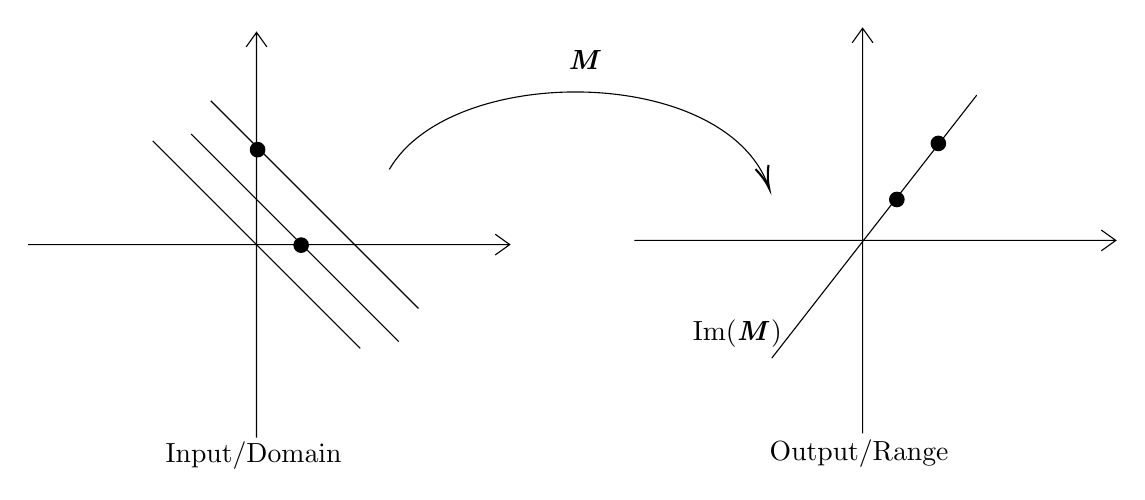
\begin{tikzpicture}[x=0.75pt,y=0.75pt,yscale=-1,xscale=1]
		\draw  (32.01,149.24) -- (264.01,149.24)(142.01,47) -- (142.01,242.24) (257.01,144.24) -- (264.01,149.24) -- (257.01,154.24) (137.01,54) -- (142.01,47) -- (147.01,54)  ;
		\draw    (110.5,96.01) -- (210.5,196.01) ;
		\draw    (120,80) -- (220,180) ;
		\draw    (92.01,99.24) -- (192.01,199.24) ;
		\draw  [fill={rgb, 255:red, 0; green, 0; blue, 0 }  ,fill opacity=1 ] (160.01,149.5) .. controls (160.01,147.57) and (161.57,146.01) .. (163.5,146.01) .. controls (165.44,146.01) and (167,147.57) .. (167,149.5) .. controls (167,151.44) and (165.44,153) .. (163.5,153) .. controls (161.57,153) and (160.01,151.44) .. (160.01,149.5) -- cycle ;
		\draw  [fill={rgb, 255:red, 0; green, 0; blue, 0 }  ,fill opacity=1 ] (139.01,103.5) .. controls (139.01,101.57) and (140.57,100.01) .. (142.5,100.01) .. controls (144.44,100.01) and (146,101.57) .. (146,103.5) .. controls (146,105.44) and (144.44,107) .. (142.5,107) .. controls (140.57,107) and (139.01,105.44) .. (139.01,103.5) -- cycle ;
		\draw  (324.01,147.24) -- (556.01,147.24)(434.01,45) -- (434.01,240.24) (549.01,142.24) -- (556.01,147.24) -- (549.01,152.24) (429.01,52) -- (434.01,45) -- (439.01,52)  ;
		\draw    (489.01,77.24) -- (390.26,203.93) ;
		\draw  [fill={rgb, 255:red, 0; green, 0; blue, 0 }  ,fill opacity=1 ] (467.01,100.5) .. controls (467.01,98.57) and (468.57,97.01) .. (470.5,97.01) .. controls (472.44,97.01) and (474,98.57) .. (474,100.5) .. controls (474,102.44) and (472.44,104) .. (470.5,104) .. controls (468.57,104) and (467.01,102.44) .. (467.01,100.5) -- cycle ;
		\draw  [fill={rgb, 255:red, 0; green, 0; blue, 0 }  ,fill opacity=1 ] (447.01,127.5) .. controls (447.01,125.57) and (448.57,124.01) .. (450.5,124.01) .. controls (452.44,124.01) and (454,125.57) .. (454,127.5) .. controls (454,129.44) and (452.44,131) .. (450.5,131) .. controls (448.57,131) and (447.01,129.44) .. (447.01,127.5) -- cycle ;
		\draw    (206,113) .. controls (235.71,61.75) and (366.37,62.45) .. (388.38,120.46) ;
		\draw [shift={(389.01,122.24)}, rotate = 251.51] [color={rgb, 255:red, 0; green, 0; blue, 0 }  ][line width=0.75]    (10.93,-3.29) .. controls (6.95,-1.4) and (3.31,-0.3) .. (0,0) .. controls (3.31,0.3) and (6.95,1.4) .. (10.93,3.29)   ;
		\draw (97,243) node [anchor=north west][inner sep=0.75pt]   [align=left] {Input/Domain};
		\draw (388,242) node [anchor=north west][inner sep=0.75pt]   [align=left] {Output/Range};
		\draw (351,184.4) node [anchor=north west][inner sep=0.75pt]    {$\text{Im}(\matrixM)$};
		\draw (291,54.4) node [anchor=north west][inner sep=0.75pt]    {$\matrixM$};
	\end{tikzpicture}
	\end{center}
\end{eg}
\begin{thm}[Invertibility Criteria]
	Let $\matrixA$ be an $n\times m$ matrix: 
	\begin{enumerate}
		\item $\matrixA$ is invertible \emph{iff} $\matrixA\vecx=\vecb$ has a unique solution $\forall\vecb\in\R^n$.
		\[\Longleftrightarrow\IM(\matrixA)=\R^n\quad\text{and}\quad\Ker(\matrixA)=\{\vec{0}\}.\]
		\[\Longleftrightarrow\rank(\matrixA)=n\quad\text{and}\quad\nullity(\matrixA)=0.\]
		\item If $\matrixA$ is an $n\times m$ matrix, then the following are equivalent: 
		\begin{enumerate}
			\item $\matrixA\vecx=\vecb$ has a unique solution for all $\vecb$ in $\R^n.$
			\item $\rank(\matrixA)=n$
			\item $\nullity(\matrixA)=0$
			\item $\IM(\matrixA)=\R^n$
			\item $\Ker(\matrixA)=\{\vec{0}\}$
			\item $\rref(\matrixA)=\matrixI_n$
			\item The columns of $\matrixA$ form a basis for $\R^n$
			\item The columns of $\matrixA$ span $\R^n$
			\item The columns of $\matrixA$ are $\LI$
			\item There is a matrix $\matrixB$ \emph{s.t.} \[\matrixB\matrixA=\matrixI=\matrixA\matrixB\qquad(\matrixB\coloneqq\matrixA^{-1})\] 
		\end{enumerate}
	\end{enumerate}
\end{thm}

\subsection{Coordinates}
\begin{rmk}[Goal of Coordinates]
	To describe the location of a vector within a subspace. 	
\end{rmk}
\begin{df}[Standard coordinates on $\R^n$]
	We can write $\vecx$ as a linear combination of the standard basis vectors. \[\text{i.e., }\vecx=a_1+\vece_1+a_2\vece_2+\cdots+a_n\vece_n;\ a_i\in\R.\]
	\begin{eg}
		Suppose $\vecx=\begin{bmatrix}1\\2\end{bmatrix}\in\R^2.$ Then $\vecx=\vece_1+2\vece_2.$	
		\begin{center}
		\tikzset{every picture/.style={line width=0.75pt}} 
		\begin{tikzpicture}[x=0.75pt,y=0.75pt,yscale=-1,xscale=1]
		\draw  (51,229.55) -- (240.01,229.55)(69.9,73) -- (69.9,246.95) (233.01,224.55) -- (240.01,229.55) -- (233.01,234.55) (64.9,80) -- (69.9,73) -- (74.9,80)  ;
		\draw  [dash pattern={on 4.5pt off 4.5pt}]  (110.01,149.77) -- (110,230) ;
		\draw  [dash pattern={on 4.5pt off 4.5pt}]  (110.01,149.77) -- (70.01,149.77) ;
		\draw  [fill={rgb, 255:red, 0; green, 0; blue, 0 }  ,fill opacity=1 ] (105.51,149.77) .. controls (105.51,147.28) and (107.53,145.27) .. (110.01,145.27) .. controls (112.49,145.27) and (114.5,147.28) .. (114.5,149.77) .. controls (114.5,152.25) and (112.49,154.26) .. (110.01,154.26) .. controls (107.53,154.26) and (105.51,152.25) .. (105.51,149.77) -- cycle ;
		\draw    (69.9,229.55) -- (108,229.98) ;
		\draw [shift={(110,230)}, rotate = 180.64] [color={rgb, 255:red, 0; green, 0; blue, 0 }  ][line width=0.75]    (10.93,-3.29) .. controls (6.95,-1.4) and (3.31,-0.3) .. (0,0) .. controls (3.31,0.3) and (6.95,1.4) .. (10.93,3.29)   ;
		\draw    (69.9,229.55) -- (70.01,151.77) ;
		\draw [shift={(70.01,149.77)}, rotate = 90.08] [color={rgb, 255:red, 0; green, 0; blue, 0 }  ][line width=0.75]    (10.93,-3.29) .. controls (6.95,-1.4) and (3.31,-0.3) .. (0,0) .. controls (3.31,0.3) and (6.95,1.4) .. (10.93,3.29)   ;
		\draw (104,236.4) node [anchor=north west][inner sep=0.75pt]    {$\vece_{1}$};
		\draw (39,144.4) node [anchor=north west][inner sep=0.75pt]    {$2\vece_{2}$};
		\draw (122,126.4) node [anchor=north west][inner sep=0.75pt]    {$\vecx =\vece_{1} +2\vece_2$};
		\end{tikzpicture}
		\end{center}
	\end{eg}
\end{df}
\begin{thm}
	Let $V\subseteq\R^n$ be a subspace and $\beta=(\vecx_1,\cdots,\vecx_m)$ be a basis. Then every $\vecx\in V$ may be written as $\vecx=a_1\vecx_1+a_2\vecx_2+\cdots+a_m\vecx_m$ for some unique scalars $a_1,\cdots,a_m\in\R.$
	\begin{eg}
		Suppose $V$ is a subspace and $\beta=(\vecx_1,\vecx_2)$: 
		\begin{center}
		\tikzset{every picture/.style={line width=0.75pt}}       
		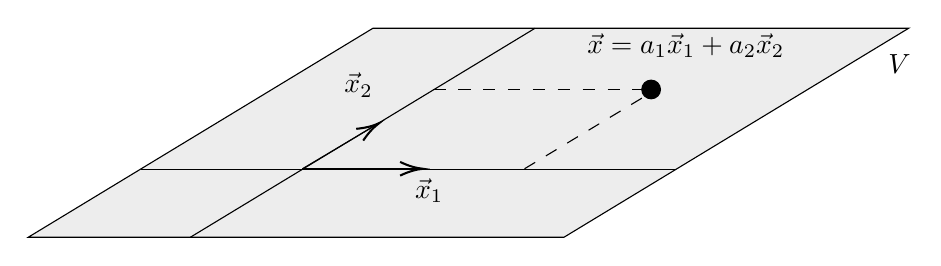
\begin{tikzpicture}[x=0.75pt,y=0.75pt,yscale=-1,xscale=1]
		\draw  [fill={rgb, 255:red, 0; green, 0; blue, 0 }  ,fill opacity=0.07 ] (279.99,102) -- (538.1,102) -- (372.01,202.71) -- (113.9,202.71) -- cycle ;
		\draw    (168,170) -- (426.01,170) ;
		\draw    (192.01,202.71) -- (358.1,102) ;
		\draw    (246.01,169.71) -- (302.01,169.71) ;
		\draw [shift={(304.01,169.71)}, rotate = 180] [color={rgb, 255:red, 0; green, 0; blue, 0 }  ][line width=0.75]    (10.93,-3.29) .. controls (6.95,-1.4) and (3.31,-0.3) .. (0,0) .. controls (3.31,0.3) and (6.95,1.4) .. (10.93,3.29)   ;
		\draw    (246.01,169.71) -- (281.29,148.73) ;
		\draw [shift={(283.01,147.71)}, rotate = 149.26] [color={rgb, 255:red, 0; green, 0; blue, 0 }  ][line width=0.75]    (10.93,-3.29) .. controls (6.95,-1.4) and (3.31,-0.3) .. (0,0) .. controls (3.31,0.3) and (6.95,1.4) .. (10.93,3.29)   ;
		\draw  [fill={rgb, 255:red, 0; green, 0; blue, 0 }  ,fill opacity=1 ] (409.51,131.5) .. controls (409.51,129.02) and (411.53,127.01) .. (414.01,127.01) .. controls (416.49,127.01) and (418.5,129.02) .. (418.5,131.5) .. controls (418.5,133.99) and (416.49,136) .. (414.01,136) .. controls (411.53,136) and (409.51,133.99) .. (409.51,131.5) -- cycle ;
		\draw  [dash pattern={on 4.5pt off 4.5pt}]  (353.01,169.71) -- (416.5,131.5) ;
		\draw  [dash pattern={on 4.5pt off 4.5pt}]  (309.01,131.5) -- (414.01,131.5) ;
		\draw (527,113.4) node [anchor=north west][inner sep=0.75pt]    {$V$};
		\draw (299,173.4) node [anchor=north west][inner sep=0.75pt]    {$\vecx_{1}$};
		\draw (265,122.4) node [anchor=north west][inner sep=0.75pt]    {$\vecx_{2}$};
		\draw (382,103.4) node [anchor=north west][inner sep=0.75pt]    {$\vecx =a_{1}\vecx_1 +a_{2}\vecx_{2}$};
		\end{tikzpicture}
		\end{center}
	\end{eg}
\end{thm}
\begin{df}[$\beta$ coordinates]
	Let	$V\subseteq\R^n$ be a subspace and $\beta$ be a basis for $V$. Let $\vecx\in V$. The $\beta$\textbf{-coordinates} for $\vecx$ in $V$ is the following vector: \[\left[\vecx\right]_\beta=\begin{bmatrix}a_1\\\vdots\\a_m\end{bmatrix}\] \emph{s.t.} $\vecx=a_1\vecx_1+\cdots+a_m\vecx_m.$
	\begin{eg}
		Suppose $V=\Span\left(\begin{bmatrix}1\\1\\0\end{bmatrix},\begin{bmatrix}0\\1\\1\end{bmatrix}\right)$ and $\beta=\left(\begin{bmatrix}1\\1\\0\end{bmatrix}, \begin{bmatrix}0\\1\\1\end{bmatrix}\right)$.\\
		Let $\vecx=2\begin{bmatrix}1\\1\\0\end{bmatrix}+1\begin{bmatrix}0\\1\\1\end{bmatrix}=\begin{bmatrix}2\\3\\1\end{bmatrix}$. 
		Then, $[\vecx]_\beta=\begin{bmatrix}2\\1\end{bmatrix}$.
	\end{eg}
	\begin{rmk} 
		$V$ in general has many basis. The $\beta$-coordinates depend on the basis. Also, in general, coordinate axes are not perpendicular. 
	\end{rmk}
\end{df}
\begin{eg}
	Let $V\subseteq\R^3$ be the subspace spanned by $\vecv_1=\begin{bmatrix}1\\2\\1\end{bmatrix},\ \vecv_2=\begin{bmatrix}-3\\2\\3\end{bmatrix}.$ Let $\beta=(\vecv_1,\vecv_2)$ and $\vecx=\begin{bmatrix}-1\\2\\2\end{bmatrix}$. Find $[\vecx]_\beta.$	\\
	\begin{sol}
		Find $[\vecx]_\beta=\begin{bmatrix}c_1\\c_2\end{bmatrix}$ \emph{s.t.} $\vecx=c_1\vecv_1+c_2\vecv_2.$ (Find an expression for $\vecx$ in the span of $\vecv_1$ and $\vecv_2$, which is the image of $\matrixS=\begin{bmatrix}|&|\\\vecv_1&\vecv_2\\|&|\end{bmatrix}$. Hence, we need to find $\vecx=\matrixS\begin{bmatrix}c_1\\c_2\end{bmatrix}$ (i.e., solve $\matrixS\vec{c}=\vecx$).\\
		Form augmented matrix $\left[\begin{array}{c:c}\matrixS&\vecx\end{array}\right]$: 
		$$\begin{aligned}
			\left[\begin{array}{c:c}\matrixS&\vecx\end{array}\right]&=\left[\begin{array}{c:c}\begin{matrix}|&|\\\vecv_1&\vecv_2\\|&|\end{matrix}&\vecx\end{array}\right]=\left[\begin{array}{c:c}\begin{matrix}1&-3\\2&2\\1&3\end{matrix}&\begin{matrix}-1\\2\\2\end{matrix}\end{array}\right]\\
			&\xRightarrow[\text{reduce}]{\text{Row}}\left[\begin{array}{c:c}\begin{matrix}1&0\\0&1\\0&0\end{matrix}&\begin{matrix}^1/_2\\^1/_2\\0\end{matrix}\end{array}\right]
		\end{aligned}$$
		\[\therefore[\vecx]_\beta=\begin{bmatrix}^1/_2\\^1/_2\\\end{bmatrix}.\]
	\end{sol}
	\begin{rmk} If $(\vecv_1,\cdots,\vecv_m)=\beta$ is a basis for a subspace $V$, and $\matrixS\coloneqq\begin{bmatrix}|&&|\\\vecv_1&\cdots&\vecv_m\\|&&|\end{bmatrix}$, then $\matrixS$ converts $\beta$-coordinates to standard coordinates. \[\text{i.e., }\matrixS[\vecx]_\beta=\vecx.\]
	\end{rmk}
\end{eg}
\begin{eg}[$\beta$-coordinates Under Linear Transformation]
	Consider $\T: \R^2\to\R^2$ defined by matrix $\begin{bmatrix}1&3\\2&2\end{bmatrix}$. Let $\vecx\in\R^2$ be the vector whose $\beta$-coordinates are $[\vecx]_\beta=\begin{bmatrix}1\\3\end{bmatrix}$, where $\beta=\left(\begin{bmatrix}1\\1\end{bmatrix},\begin{bmatrix}1\\-1\end{bmatrix}\right)$. Find $[\T\vecx]_\beta$.\\
	\begin{sol}
		First, unpack the question: 
		\begin{center}
		\tikzset{every picture/.style={line width=0.75pt}} 
		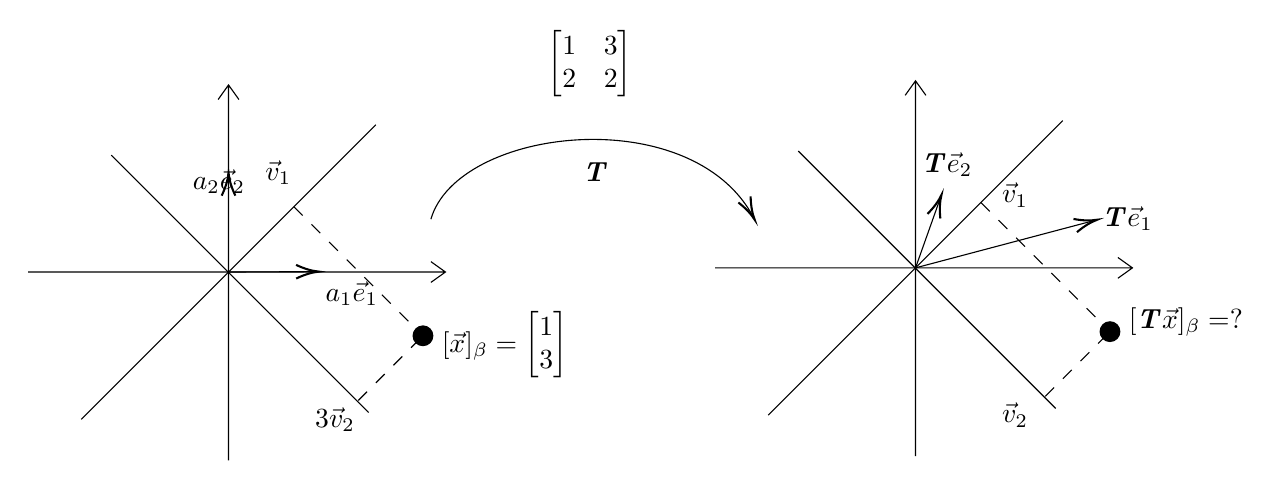
\begin{tikzpicture}[x=0.75pt,y=0.75pt,yscale=-1,xscale=1]
		\draw  (44,147.46) -- (245.01,147.46)(140.5,57.34) -- (140.5,238.18) (238.01,142.46) -- (245.01,147.46) -- (238.01,152.46) (135.5,64.34) -- (140.5,57.34) -- (145.5,64.34)  ;
		\draw    (211.46,76.5) -- (69.55,218.42) ;
		\draw    (84.01,91.18) -- (208.01,215.18) ;
		\draw  [dash pattern={on 4.5pt off 4.5pt}]  (172,116) -- (234.18,178.18) ;
		\draw  [dash pattern={on 4.5pt off 4.5pt}]  (203.01,209.35) -- (234.18,178.18) ;
		\draw  [fill={rgb, 255:red, 0; green, 0; blue, 0 }  ,fill opacity=1 ] (229.43,178.18) .. controls (229.43,175.56) and (231.56,173.43) .. (234.18,173.43) .. controls (236.8,173.43) and (238.93,175.56) .. (238.93,178.18) .. controls (238.93,180.8) and (236.8,182.93) .. (234.18,182.93) .. controls (231.56,182.93) and (229.43,180.8) .. (229.43,178.18) -- cycle ;
		\draw  (375,145.46) -- (576.01,145.46)(471.5,55.34) -- (471.5,236.18) (569.01,140.46) -- (576.01,145.46) -- (569.01,150.46) (466.5,62.34) -- (471.5,55.34) -- (476.5,62.34)  ;
		\draw    (542.46,74.5) -- (400.55,216.42) ;
		\draw    (415.01,89.18) -- (539.01,213.18) ;
		\draw  [dash pattern={on 4.5pt off 4.5pt}]  (503,114) -- (565.18,176.18) ;
		\draw  [dash pattern={on 4.5pt off 4.5pt}]  (534.01,207.35) -- (565.18,176.18) ;
		\draw  [fill={rgb, 255:red, 0; green, 0; blue, 0 }  ,fill opacity=1 ] (560.43,176.18) .. controls (560.43,173.56) and (562.56,171.43) .. (565.18,171.43) .. controls (567.8,171.43) and (569.93,173.56) .. (569.93,176.18) .. controls (569.93,178.8) and (567.8,180.93) .. (565.18,180.93) .. controls (562.56,180.93) and (560.43,178.8) .. (560.43,176.18) -- cycle ;
		\draw    (238,122) .. controls (250.88,77.72) and (362.75,64.79) .. (393.11,120.56) ;
		\draw [shift={(394.01,122.27)}, rotate = 243.34] [color={rgb, 255:red, 0; green, 0; blue, 0 }  ][line width=0.75]    (10.93,-3.29) .. controls (6.95,-1.4) and (3.31,-0.3) .. (0,0) .. controls (3.31,0.3) and (6.95,1.4) .. (10.93,3.29)   ;
		\draw    (140.5,147.46) -- (140.5,101.73) ;
		\draw [shift={(140.5,99.73)}, rotate = 90] [color={rgb, 255:red, 0; green, 0; blue, 0 }  ][line width=0.75]    (10.93,-3.29) .. controls (6.95,-1.4) and (3.31,-0.3) .. (0,0) .. controls (3.31,0.3) and (6.95,1.4) .. (10.93,3.29)   ;
		\draw    (140.5,147.46) -- (182.01,147.28) ;
		\draw [shift={(184.01,147.27)}, rotate = 179.75] [color={rgb, 255:red, 0; green, 0; blue, 0 }  ][line width=0.75]    (10.93,-3.29) .. controls (6.95,-1.4) and (3.31,-0.3) .. (0,0) .. controls (3.31,0.3) and (6.95,1.4) .. (10.93,3.29)   ;
		\draw    (471.5,145.46) -- (557.08,122.78) ;
		\draw [shift={(559.01,122.27)}, rotate = 165.15] [color={rgb, 255:red, 0; green, 0; blue, 0 }  ][line width=0.75]    (10.93,-3.29) .. controls (6.95,-1.4) and (3.31,-0.3) .. (0,0) .. controls (3.31,0.3) and (6.95,1.4) .. (10.93,3.29)   ;
		\draw    (471.5,145.46) -- (483.34,112.15) ;
		\draw [shift={(484.01,110.27)}, rotate = 109.56] [color={rgb, 255:red, 0; green, 0; blue, 0 }  ][line width=0.75]    (10.93,-3.29) .. controls (6.95,-1.4) and (3.31,-0.3) .. (0,0) .. controls (3.31,0.3) and (6.95,1.4) .. (10.93,3.29)   ;
		\draw (157,92.4) node [anchor=north west][inner sep=0.75pt]    {$\vecv_{1}$};
		\draw (181,211.4) node [anchor=north west][inner sep=0.75pt]    {$3\vecv_{2}$};
		\draw (242,165.4) node [anchor=north west][inner sep=0.75pt]    {$[\vecx]_{\beta } =\begin{bmatrix}1\\3\end{bmatrix}$};
		\draw (512,103.4) node [anchor=north west][inner sep=0.75pt]    {$\vecv_{1}$};
		\draw (512,209.4) node [anchor=north west][inner sep=0.75pt]    {$\vecv_{2}$};
		\draw (573,163.4) node [anchor=north west][inner sep=0.75pt]    {$[ \T \vec{x}]_{\beta } =?$};
		\draw (293,30) node [anchor=north west][inner sep=0.75pt]    {$\begin{bmatrix}1 & 3\\2 & 2\end{bmatrix}$};
		\draw (310,93.4) node [anchor=north west][inner sep=0.75pt]    {$\T $};
		\draw (186.01,150.67) node [anchor=north west][inner sep=0.75pt]    {$a_1\vece_{1}$};
		\draw (122.01,96.67) node [anchor=north west][inner sep=0.75pt]    {$a_2\vece_{2}$};
		\draw (560.01,114.67) node [anchor=north west][inner sep=0.75pt]    {$\T \vec{e}_{1}$};
		\draw (473.01,88.67) node [anchor=north west][inner sep=0.75pt]    {$\T \vec{e}_{2}$};
		\end{tikzpicture}
		\end{center}
		To solve this question: 
		\begin{enumerate}
			\item Find standard coordinates for $\vecx$: 
				\[\matrixS=\begin{bmatrix}1&1\\1&-1\end{bmatrix}\Longrightarrow[\vecx]_{st}=\matrixS[\vecx]_\beta=\begin{bmatrix}1&1\\1&-1\end{bmatrix}\begin{bmatrix}1\\3\end{bmatrix}=\begin{bmatrix}4\\-2\end{bmatrix}\]
			\item Multiply $[\vecx]_{st}$ by $\T$: 
				\[\T[\vecx]_{st}=\begin{bmatrix}1 & 3\\2 & 2\end{bmatrix}\begin{bmatrix}4\\-2\end{bmatrix}=\begin{bmatrix}-2\\-4\end{bmatrix}\]
			\item Compute $[\T\vecx]_\beta$.
				\[\T[\vecx]_{st}=\matrixS[\T\vecx]_\beta\Longrightarrow\begin{bmatrix}-2\\-4\end{bmatrix}=\begin{bmatrix}1&1\\1&-1\end{bmatrix}[\T\vecx]_\beta\Longrightarrow[\T\vecx]_\beta=\begin{bmatrix}1\\3\end{bmatrix}.\]
		\end{enumerate}
	\end{sol}
\end{eg}
\begin{thm}
	Let $\T: \R^n\to\R^m$ be a linear transformation and $\beta=(\vecv_1,\cdots,\vecv_n)$ be a basis for $\R^n$. Let $\vecx\in\R^n$: \[[\T\vecx]_\beta=\matrixS^{-1}\T\matrixS[\vecx]_\beta,\qquad\text{where}\quad\matrixS=\begin{bmatrix}|&&|\\\vecv_1&\cdots&\vecv_n\\|&&|\end{bmatrix}.\] 	\[[\T\vecx]_\beta=[\T]_\beta[\vecx]_\beta.\]
\end{thm}
\begin{thm}
	The matrix for $\T$ with respect to the basis $\beta$ is \[[\T]_\beta=\matrixS^{-1}\T\matrixS.\]	
	\begin{eg}
		Let $\T=\begin{bmatrix}1&3\\2&2\end{bmatrix}$ and $\beta=\left(\begin{bmatrix}1\\1\end{bmatrix},\begin{bmatrix}1\\-1\end{bmatrix}\right)$. Then \[[\T]_\beta=\begin{bmatrix}^1/_2&^1/_2\\^1/_2&-^1/_2\end{bmatrix}\begin{bmatrix}1&3\\2&2\end{bmatrix}\begin{bmatrix}1&1\\1&-1\end{bmatrix}=\begin{bmatrix}4&-1\\0&-1\end{bmatrix}.\]
	\end{eg}
\end{thm}

\newpage
\section{Approximate Solution of $\matrixA\vecx=\vecb$}
\subsection{Lengths and Angles in $\R^n$}
\begin{df}[Dot Product]
	Let $\vecx=\begin{bmatrix}x_1\\\vdots\\x_n\end{bmatrix}$ and $\vecy=\begin{bmatrix}y_1\\\vdots\\y_n\end{bmatrix}\in\R^n$. The \textbf{dot product} of $\vecx$ and $\vecy$ is the following number: \[\vecx\cdot\vecy=\begin{bmatrix}x_1\\\vdots\\x_n\end{bmatrix}\cdot\begin{bmatrix}y_1\\\vdots\\y_n\end{bmatrix}=x_1y_1+x_2y_2+\cdots+x_ny_n=\begin{bmatrix}x_1&\cdots&x_n\end{bmatrix}\begin{bmatrix}y_1\\\vdots\\y_n\end{bmatrix}\]	
	\begin{eg}
		\[\begin{bmatrix}1\\2\\3\end{bmatrix}\cdot\begin{bmatrix}7\\5\\2\end{bmatrix}=1\times7+2\times5+3\times2=23.\]	
	\end{eg}
\end{df}
\begin{thm}
	Algebraic property of dot products:
	\begin{enumerate}
		\item $\vecx\cdot\vecy=\vecy\cdot\vecx$
		\item $\vecx\cdot(\vecy_1+\vecy_2)=\vecx\cdot\vecy_1+\vecx\cdot\vecy_2$\\
			$(\vecx_1+\vecx_2)\cdot\vecy=\vecx_1\cdot\vecy+\vecx_2\cdot\vecy$
		\item $\vecx\cdot(c\vecy)=c(\vecx\cdot\vecy)=(c\vecx)\cdot\vecy$
	\end{enumerate}
\end{thm}
\begin{df}[Length]
	Let $\vecx\in\R^n$. The \textbf{length} of $\vecx$ is the following number: 
	\[\|\vecx\|\coloneqq\sqrt{\vecx\cdot\vecx}=\sqrt{x_1^2+x_2^2+\cdots+x_n^2},\text{ where }\vecx=\begin{bmatrix}x_1\\\vdots\\x_n\end{bmatrix}\]	
	\begin{eg}
		\[\left\|\begin{bmatrix}4\\3\end{bmatrix}\right\|=\sqrt{4^2+3^2}=5\]
		\begin{rmk}
			In $\R^2$, the definition of length is the Pythagorean theorem.	
		\end{rmk}
	\end{eg}
\end{df}
\begin{thm}[Angle Between Vectors]
	Let $\theta$ be the angle between $\vecx$ and $\vecy$. We then have \[\cos\theta=\frac{\|\vecx\|^2+\|\vecy\|^2-\|\vecy-\vecx\|^2}{2\|\vecx\|\|\vecy\|}\]
	\begin{prf}
		Assume vectors $\vecx$ and $\vecy$ are drawn as below. 
		\begin{center}
		\tikzset{every picture/.style={line width=0.75pt}} 
		\begin{tikzpicture}[x=0.75pt,y=0.75pt,yscale=-1,xscale=1]
		\draw    (148.62,95.54) -- (36.01,212.1) ;
		\draw [shift={(150.01,94.1)}, rotate = 134.01] [color={rgb, 255:red, 0; green, 0; blue, 0 }  ][line width=0.75]    (10.93,-3.29) .. controls (6.95,-1.4) and (3.31,-0.3) .. (0,0) .. controls (3.31,0.3) and (6.95,1.4) .. (10.93,3.29)   ;
		\draw    (171.14,264.38) -- (36.01,212.1) ;
		\draw [shift={(173.01,265.1)}, rotate = 201.15] [color={rgb, 255:red, 0; green, 0; blue, 0 }  ][line width=0.75]    (10.93,-3.29) .. controls (6.95,-1.4) and (3.31,-0.3) .. (0,0) .. controls (3.31,0.3) and (6.95,1.4) .. (10.93,3.29)   ;
		\draw    (173.01,265.1) -- (150.01,94.1) ;
		\draw (50,199.4) node [anchor=north west][inner sep=0.75pt]    {$\theta $};
		\draw (69,135.4) node [anchor=north west][inner sep=0.75pt]    {$\| \vec{x} \| $};
		\draw (79,238.4) node [anchor=north west][inner sep=0.75pt]    {$\| \vec{y} \| $};
		\draw (137,75.4) node [anchor=north west][inner sep=0.75pt]    {$\vec{x}$};
		\draw (175.01,268.5) node [anchor=north west][inner sep=0.75pt]    {$\vec{y}$};
		\draw (167,173.4) node [anchor=north west][inner sep=0.75pt]    {$L=\| \vec{y} -\vec{x} \| $};
		\end{tikzpicture}
		\end{center}
		By the cosine rule, we have:
		\[L^2=\|\vecx\|^2+\|\vecy\|^2-2\|\vecx\|\|\vecy\|\cos\theta\]
		So, \[\cos\theta=\frac{\|\vecx\|^2+\|\vecy\|^2-L^2}{2\|\vecx\|\|\vecy\|}=\frac{\|\vecx\|^2+\|\vecy\|^2-\|\vecy-\vecx\|^2}{2\|\vecx\|\|\vecy\|}.\]
	\end{prf}
\end{thm}
\begin{thm}
	Relationship of angle and dot products:
	\begin{enumerate}
		\item $\vecx\cdot\vecy>0$ if $\theta<90^\circ$
		\item $\vecx\cdot\vecy=0$ if $\theta=90^\circ$	
		\item $\vecx\cdot\vecy<0$ if $\theta>90^\circ$
	\end{enumerate}
	\begin{prf}
		$$\begin{aligned}
			\|\vecy-\vecx\|^2&=(\vecy-\vecx)\cdot(\vecy-\vecx)\\
			&=(\vecy-\vecx)\cdot\vecy-(\vecy-\vecx)\cdot\vecx\\
			&=\vecy\cdot\vecy-\vecx\cdot\vecy-\vecy\cdot\vecx+\vecx\cdot\vecx\\
			&=\vecy\cdot\vecy-2\vecx\cdot\vecy+\vecx\cdot\vecx\\
			&=\|\vecy\|^2-2\vecx\cdot\vecy+\|\vecx\|^2
		\end{aligned}$$
		Think of Pythagonean theorem: 
		\begin{center}
			\tikzset{every picture/.style={line width=0.75pt}}
			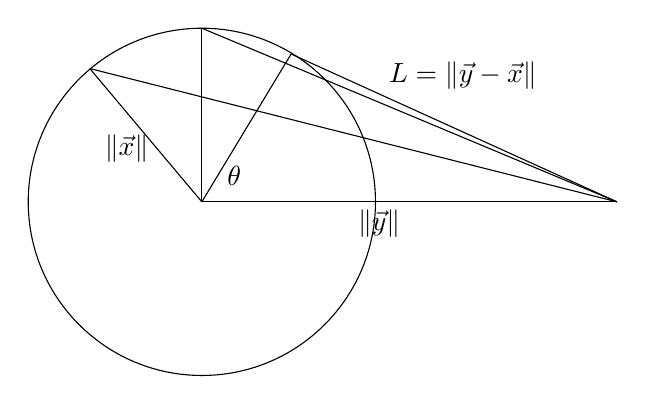
\begin{tikzpicture}[x=0.75pt,y=0.75pt,yscale=-1,xscale=1]
			\draw    (211,180) -- (411.01,180) ;
			\draw    (211,96.35) -- (211,180) ;
			\draw   (127.35,180) .. controls (127.35,133.8) and (164.8,96.35) .. (211,96.35) .. controls (257.2,96.35) and (294.65,133.8) .. (294.65,180) .. controls (294.65,226.2) and (257.2,263.65) .. (211,263.65) .. controls (164.8,263.65) and (127.35,226.2) .. (127.35,180) -- cycle ;
			\draw    (157.01,115.77) -- (211,180) ;
			\draw    (254.01,108.77) -- (211,180) ;
			\draw    (254.01,108.77) -- (411.01,180) ;
			\draw    (211,96.35) -- (411.01,180) ;
			\draw    (157.01,115.77) -- (411.01,180) ;
			\draw (222,161.4) node [anchor=north west][inner sep=0.75pt]    {$\theta $};
			\draw (285,182.4) node [anchor=north west][inner sep=0.75pt]    {$\| \vec{y} \| $};
			\draw (163,146.4) node [anchor=north west][inner sep=0.75pt]    {$\| \vec{x} \| $};
			\draw (300,111.4) node [anchor=north west][inner sep=0.75pt]    {$L=\| \vec{y} -\vec{x} \| $};
			\end{tikzpicture}
		\end{center}
		\begin{itemize}
			\item If $\theta<90^\circ,\ \|\vecy-\vecx\|^2<\|\vecy\|+\|\vec\|^2\Longrightarrow\vecx\cdot\vecy>0.$	
			\item If $\theta=90^\circ,\ \|\vecy-\vecx\|^2=\|\vecy\|+\|\vec\|^2\Longrightarrow\vecx\cdot\vecy=0.$	
			\item If $\theta>90^\circ,\ \|\vecy-\vecx\|^2>\|\vecy\|+\|\vec\|^2\Longrightarrow\vecx\cdot\vecy<0.$	
		\end{itemize}
	\end{prf}
\end{thm}
\begin{df}[Perpendicular]
	Let $\vecx,\vecy\in\R^n$. Then, $\vecx$ and $\vecy$ are \textbf{perpendicular} \emph{iff} $\vecx\cdot\vecy=0$. (Equivalently: orthogonal)	
\end{df}
\begin{thm}
	Suppose $\matrixA$ is an $1\times n$ matrix \emph{s.t.} $\matrixA=\begin{bmatrix}a_1&\cdots&a_n\end{bmatrix}.$ Then, $\matrixA^\T=\begin{bmatrix}a_1\\\vdots\\a_n\end{bmatrix}=\vecv$. Thus, 	$\matrixA\vecx=\vecv\cdot\vecx$.
\end{thm}
\begin{thm}
	\[\vecv\perp\vecx\Longleftrightarrow\vecv\cdot\vecx=0\Longleftrightarrow\matrixA\vecx=0\Longrightarrow\vecx\in\Ker(\matrixA).\]	
	\begin{itemize}
		\item Let $\vecv\neq\vec{0}$. The set $\{\vecx\ |\ \vecx\perp\vecv\}$ is a subspace of dimension $m-1$.
		\item Let $\matrixA: \R^m\to\R^n$ be a linear transformation. Then, the kernel of $\matrixA$ is the set of all vectors $\vecx\in\R^m$, which are perpendicular to the row of the matrix for $\matrixA$.
	\end{itemize}
\end{thm}
\begin{thm}
	\[\vecx\cdot\vecv=\|\vecx\|\|\vecv\|\cos\theta\]
	\begin{prf}
		\begin{enumerate}
			\item $\vecv\cdot\vecx$ is constant along translates of the subspace perpendicular to the line spanned by $\vecv$: \[\vecv\cdot\vecx=\matrixA\vecx=\vecb\]
			\item Project $\vecx$ into the line spanned by $\vecv$: 
			\begin{center}
			\tikzset{every picture/.style={line width=0.75pt}} 
			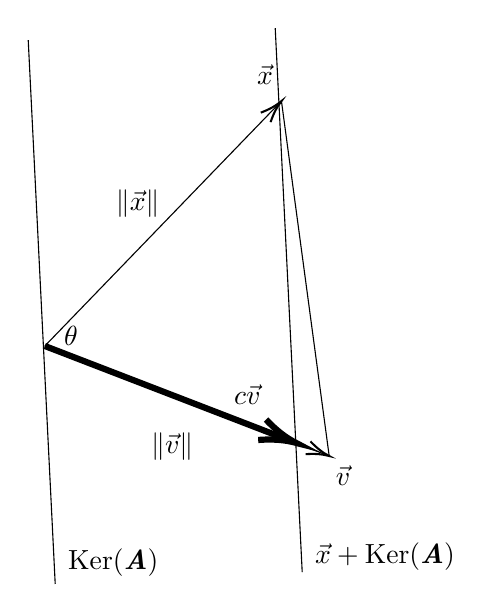
\begin{tikzpicture}[x=0.75pt,y=0.75pt,yscale=-1,xscale=1]
			\draw    (152.62,63.54) -- (40.01,180.1) ;
			\draw [shift={(154.01,62.1)}, rotate = 134.01] [color={rgb, 255:red, 0; green, 0; blue, 0 }  ][line width=0.75]    (10.93,-3.29) .. controls (6.95,-1.4) and (3.31,-0.3) .. (0,0) .. controls (3.31,0.3) and (6.95,1.4) .. (10.93,3.29)   ;
			\draw    (175.14,232.38) -- (40.01,180.1) ;
			\draw [shift={(177.01,233.1)}, rotate = 201.15] [color={rgb, 255:red, 0; green, 0; blue, 0 }  ][line width=0.75]    (10.93,-3.29) .. controls (6.95,-1.4) and (3.31,-0.3) .. (0,0) .. controls (3.31,0.3) and (6.95,1.4) .. (10.93,3.29)   ;
			\draw    (177.01,233.1) -- (154.01,62.1) ;
			\draw    (32.01,32.76) -- (45.01,294.76) ;
			\draw    (151.01,27) -- (164.01,289) ;
			\draw [line width=2.25]    (40.01,180.1) -- (157.28,225.32) ;
			\draw [shift={(161.01,226.76)}, rotate = 201.09] [color={rgb, 255:red, 0; green, 0; blue, 0 }  ][line width=2.25]    (17.49,-5.26) .. controls (11.12,-2.23) and (5.29,-0.48) .. (0,0) .. controls (5.29,0.48) and (11.12,2.23) .. (17.49,5.26)   ;
			\draw (73,103.4) node [anchor=north west][inner sep=0.75pt]    {$\| \vec{x} \| $};
			\draw (90,220.4) node [anchor=north west][inner sep=0.75pt]    {$\| \vec{v} \| $};
			\draw (141,43.4) node [anchor=north west][inner sep=0.75pt]    {$\vec{x}$};
			\draw (179.01,236.5) node [anchor=north west][inner sep=0.75pt]    {$\vec{v}$};
			\draw (50,276.4) node [anchor=north west][inner sep=0.75pt]    {$\Ker(\matrixA)$};
			\draw (169,273.4) node [anchor=north west][inner sep=0.75pt]    {$\vec{x} +\Ker(\matrixA)$};
			\draw (48,169.4) node [anchor=north west][inner sep=0.75pt]    {$\theta $};
			\draw (130,197.4) node [anchor=north west][inner sep=0.75pt]    {$c\vec{v}$};
			\end{tikzpicture}
			\end{center}
			\item Use trigonometry to calculate the projection: 
				\[c\vecv=(\|\vecx\|\cos\theta)\left(\frac{\vecv}{\|\vecv\|}\right)\]
				$$\begin{aligned}
					\vecv\cdot\vecx&=\vecv\cdot c\vecv\\
					&=\frac{\|\vecx\|\cos\theta}{\|\vecv\|}\|\vecv\|^2=\|\vecx\|\cdot\|\vecv\|\cos\theta\\
					&\Rightarrow\ \theta=\arccos\left(\frac{\vecx\vecv}{\|\vecx\|\|\vecv\|}\right)
				\end{aligned}$$
		\end{enumerate}
	\end{prf}
\end{thm}
\begin{thm}
	Projection of $\vecx$ into line spanned by $\vecv$ is given by the following formula: 
	$$\begin{aligned}
		\text{Projection}=c\vecv&=\frac{\|\vecx\|\cos\theta}{\|\vecv\|}\vecv\\
		&=\frac{\vecx\cdot\vecv}{\|\vecv\|^2}\vecv\\
		&=\frac{\vecx\cdot\vecv}{\vecv\cdot\vecv}\vecv.
	\end{aligned}$$	
\end{thm}
\begin{df}[Orthogonal Complement]
	Let $V\subseteq\R^n$ be a subspace. The \textbf{orthogonal complement} of $V$ is the set of vectors perpendicular to all vectors in $V$: 
	\[V^\perp=\left\{\vecx\in\R^n;\ \vecv\cdot\vecx=0\quad\forall\vecv\in\R^n\right\}.\]	
	\begin{eg} The orthogonal complement of a line with a slope $m$ through the origin is a line through the origin with a slop of $-\dfrac{1}{m}$. \end{eg}
\end{df}
\begin{thm}
	Let $V$ be a subspace. If $\vecv_1,\cdots,\vecv_k\in V$ is a spanning set, (i.e., $V=\Span(\vecv_1,\cdots,\vecv_k)$), then $\vecx\in V^\perp$ \emph{iff} $\vecv_1\cdot\vecx=0,\ \vecv_2\cdot\vecx=0,\cdots,\vecv_k\cdot\vecx=0.$\\
	\begin{prf}
		``Perpendicular to everything'' implies $\vecv_i\cdot\vecx=0\quad\forall\vecv\in V$, then $\vecv=c_1\vecv_1+\cdots+c_k\vecv_k\Longrightarrow\vecx\cdot\vecv=c_1(\vecx\cdot\vecv_1)+\cdots+c_k(\vecx\cdot\vecv_k)=0\Longrightarrow\therefore\vecx\perp\vecv.$
	\end{prf}
\end{thm}
\begin{thm}
	Let $V\subseteq\R^n$ be a subspace, $V^\perp$ is a subspace. Specifically, if $V=\Span(\vecv_1,\cdots,\vecv_k)$, then \[V^\perp=\Ker\left(\begin{bmatrix}-&\vecv_1&-\\-&\vecv_2&-\\&\vdots&\\-&\vecv_k&-\end{bmatrix}\right)\]
	\begin{prf}
		\[\begin{bmatrix}-&\vecv_1&-\\-&\vecv_2&-\\&\vdots&\\-&\vecv_k&-\end{bmatrix}\begin{bmatrix}|\\\vecx\\|\end{bmatrix}=\begin{bmatrix}\vecx\cdot\vecv_1\\\vdots\\\vecx\cdot\vecv_k\end{bmatrix}=\begin{bmatrix}0\\\vdots\\0\end{bmatrix}\]	
	\end{prf}
	\begin{eg}
		Let $V=\Span\left(\begin{bmatrix}1\\0\\1\\1\end{bmatrix},\begin{bmatrix}1\\-1\\0\\1\end{bmatrix}\right)$. Compute $V^\perp$.	
	\begin{sol}
		\[\begin{bmatrix}1&0	&1&1\\1&-1&0&1\end{bmatrix}\xRightarrow[\text{reduce}]{\text{Row}}\begin{bmatrix}1&0&1&1\\0&-1&-1&0\end{bmatrix}\Longrightarrow\rref=\begin{bmatrix}1&0&1&1\\0&1&1&0\end{bmatrix}\]
		Unpack, we have \[\begin{cases}x_1=-x_3-x_4\\x_2=-x_3\end{cases}\]
		\[\therefore V^\perp=\text{Kernel}=\left\{\begin{bmatrix}-x_3-x_4\\-x_3\\x_3\\x_4\end{bmatrix};\ x_{3,4}\in\R\right\}=\Span\left(\begin{bmatrix}-1\\-1\\1\\0\end{bmatrix},\begin{bmatrix}-1\\0\\0\\1\end{bmatrix}\right)\]
	\end{sol}
	\end{eg}
\end{thm}

\subsection{Orthogonal Projection}
\begin{thm}
	Let $V\subseteq\R^n$ be a subspace and $\vecx\in\R^n$. Then, $\vecx$ can be written uniquely as \[\vecx=\vecx^\parallel+\vecx^\perp, \] 	when $\vecx^\parallel\in V$ and $\vecx^\perp\in V$.
\end{thm}
\begin{df}[Orthogonal Projection]
	Let $V\subseteq\R^n$ be a subspace. The \textbf{orthogonal projection} of $\vecx$ into $V$ is the vector $\vecx^\parallel$. The map $\vecx\mapsto\vecx^\parallel$ is denoted as $\Proj_V:\R^n\to\R^n$.	
\end{df}
\begin{thm}
	Computing $\Proj_V(\vecx)\coloneqq\vecx^\parallel$: 
	\begin{enumerate}
		\item Let $\vecv_1,\cdots,\vecv_k$ be a basis for $V$: \[\matrixA^\T=\begin{bmatrix}-&\vecv_1&-\\&\vdots&\\-&\vecv_k&-\end{bmatrix}\quad\text{and}\quad\matrixA=\begin{bmatrix}|&&|\\\vecv_1&cdots&\vecv_k\\|&&|\end{bmatrix}\]
		\[\boxed{\matrixA^\T\vecx^\parallel=\matrixA^\T\vecx}\]
		\begin{center}
		\tikzset{every picture/.style={line width=0.75pt}} 
		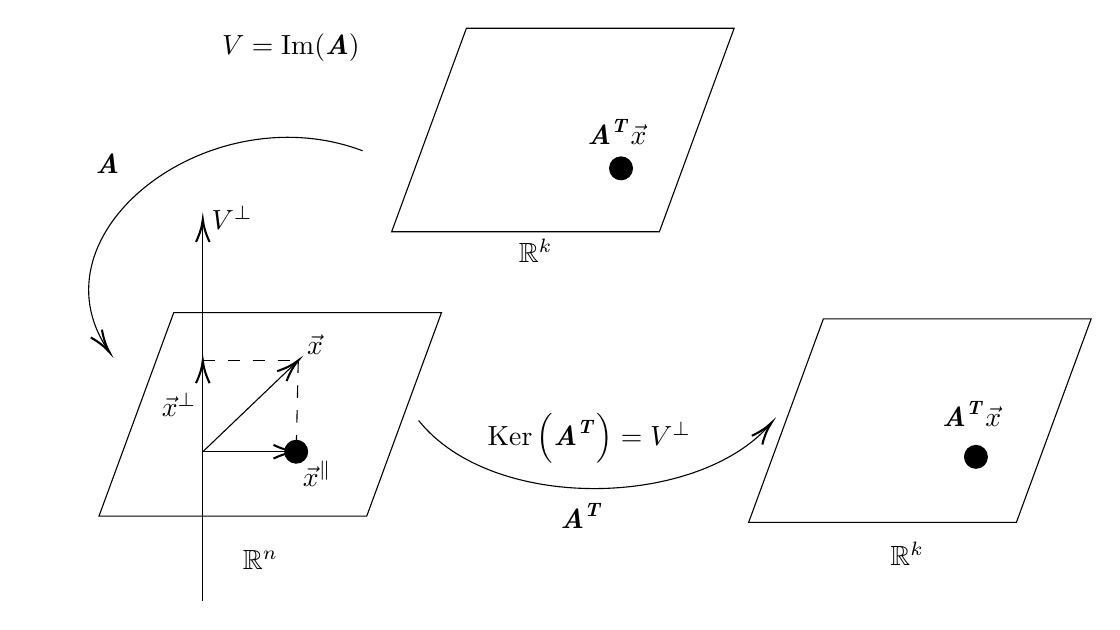
\begin{tikzpicture}[x=0.75pt,y=0.75pt,yscale=-1,xscale=1]
		\draw   (252.01,11) -- (381.01,11) -- (345,109.05) -- (216,109.05) -- cycle ;
		\draw   (111.01,148) -- (240.01,148) -- (204,246.05) -- (75,246.05) -- cycle ;
		\draw    (202.01,70.05) .. controls (128.38,42.19) and (40.9,109.42) .. (79.42,166.19) ;
		\draw [shift={(80.01,167.05)}, rotate = 234.92] [color={rgb, 255:red, 0; green, 0; blue, 0 }  ][line width=0.75]    (10.93,-3.29) .. controls (6.95,-1.4) and (3.31,-0.3) .. (0,0) .. controls (3.31,0.3) and (6.95,1.4) .. (10.93,3.29)   ;
		\draw  [fill={rgb, 255:red, 0; green, 0; blue, 0 }  ,fill opacity=1 ] (321.01,78.5) .. controls (321.01,75.47) and (323.47,73.01) .. (326.5,73.01) .. controls (329.54,73.01) and (332,75.47) .. (332,78.5) .. controls (332,81.54) and (329.54,84) .. (326.5,84) .. controls (323.47,84) and (321.01,81.54) .. (321.01,78.5) -- cycle ;
		\draw   (424.01,151) -- (553.01,151) -- (517,249.05) -- (388,249.05) -- cycle ;
		\draw  [fill={rgb, 255:red, 0; green, 0; blue, 0 }  ,fill opacity=1 ] (492.01,217.5) .. controls (492.01,214.47) and (494.47,212.01) .. (497.5,212.01) .. controls (500.54,212.01) and (503,214.47) .. (503,217.5) .. controls (503,220.54) and (500.54,223) .. (497.5,223) .. controls (494.47,223) and (492.01,220.54) .. (492.01,217.5) -- cycle ;
		\draw    (125.01,287.05) -- (125.01,105.05) ;
		\draw [shift={(125.01,103.05)}, rotate = 90] [color={rgb, 255:red, 0; green, 0; blue, 0 }  ][line width=0.75]    (10.93,-3.29) .. controls (6.95,-1.4) and (3.31,-0.3) .. (0,0) .. controls (3.31,0.3) and (6.95,1.4) .. (10.93,3.29)   ;
		\draw    (125.01,215.05) -- (169.56,172.43) ;
		\draw [shift={(171.01,171.05)}, rotate = 136.27] [color={rgb, 255:red, 0; green, 0; blue, 0 }  ][line width=0.75]    (10.93,-3.29) .. controls (6.95,-1.4) and (3.31,-0.3) .. (0,0) .. controls (3.31,0.3) and (6.95,1.4) .. (10.93,3.29)   ;
		\draw  [dash pattern={on 4.5pt off 4.5pt}]  (125.01,171.05) -- (171.01,171.05) ;
		\draw    (125.01,215.05) -- (168.01,215.05) ;
		\draw [shift={(170.01,215.05)}, rotate = 180] [color={rgb, 255:red, 0; green, 0; blue, 0 }  ][line width=0.75]    (10.93,-3.29) .. controls (6.95,-1.4) and (3.31,-0.3) .. (0,0) .. controls (3.31,0.3) and (6.95,1.4) .. (10.93,3.29)   ;
		\draw  [dash pattern={on 4.5pt off 4.5pt}]  (171.01,171.05) -- (170.01,215.05) ;
		\draw    (125.01,215.05) -- (125.01,173.05) ;
		\draw [shift={(125.01,171.05)}, rotate = 90] [color={rgb, 255:red, 0; green, 0; blue, 0 }  ][line width=0.75]    (10.93,-3.29) .. controls (6.95,-1.4) and (3.31,-0.3) .. (0,0) .. controls (3.31,0.3) and (6.95,1.4) .. (10.93,3.29)   ;
		\draw    (229,200) .. controls (264.65,244.6) and (363.02,242.1) .. (397.97,202.27) ;
		\draw [shift={(399.01,201.05)}, rotate = 129.67] [color={rgb, 255:red, 0; green, 0; blue, 0 }  ][line width=0.75]    (10.93,-3.29) .. controls (6.95,-1.4) and (3.31,-0.3) .. (0,0) .. controls (3.31,0.3) and (6.95,1.4) .. (10.93,3.29)   ;
		\draw  [fill={rgb, 255:red, 0; green, 0; blue, 0 }  ,fill opacity=1 ] (164.51,215.05) .. controls (164.51,212.01) and (166.98,209.55) .. (170.01,209.55) .. controls (173.04,209.55) and (175.5,212.01) .. (175.5,215.05) .. controls (175.5,218.08) and (173.04,220.54) .. (170.01,220.54) .. controls (166.98,220.54) and (164.51,218.08) .. (164.51,215.05) -- cycle ;
		\draw (133,12.4) node [anchor=north west][inner sep=0.75pt]    {$V=\IM(\matrixA)$};
		\draw (72,70.4) node [anchor=north west][inner sep=0.75pt]    {$\matrixA$};
		\draw (309,53.4) node [anchor=north west][inner sep=0.75pt]    {$\matrixA^{\T}\vec{x}$};
		\draw (480,189.4) node [anchor=north west][inner sep=0.75pt]    {$\matrixA^{\T}\vec{x}$};
		\draw (128,95.4) node [anchor=north west][inner sep=0.75pt]    {$V^{\perp }$};
		\draw (174,157.4) node [anchor=north west][inner sep=0.75pt]    {$\vec{x}$};
		\draw (172.01,218.45) node [anchor=north west][inner sep=0.75pt]    {$\vec{x}^{\parallel }$};
		\draw (143,261.4) node [anchor=north west][inner sep=0.75pt]    {$\mathbb{R}^{n}$};
		\draw (276,111.4) node [anchor=north west][inner sep=0.75pt]    {$\mathbb{R}^{k}$};
		\draw (455,257.4) node [anchor=north west][inner sep=0.75pt]    {$\mathbb{R}^{k}$};
		\draw (104.01,185.45) node [anchor=north west][inner sep=0.75pt]    {$\vec{x}^{\perp }$};
		\draw (296,238.4) node [anchor=north west][inner sep=0.75pt]    {$\matrixA^{\T}$};
		\draw (261,195.4) node [anchor=north west][inner sep=0.75pt]    {$\Ker\left( \matrixA^{\T}\right) =V^{\perp }$};
		\end{tikzpicture}
		\end{center}
		\item Slove $\matrixA^\T\matrixA\vec{c}=\matrixA^\T\vecx$ for $\vec{c}$.
		\item $\vecx^\parallel=\matrixA\vec{c}$
	\end{enumerate}	
	\begin{eg}
		Let $V=\Span\left(\begin{bmatrix}1\\1\\0\end{bmatrix},\begin{bmatrix}0\\1\\1\end{bmatrix}\right)$ and $\vecx=\begin{bmatrix}1\\2\\3\end{bmatrix}$. Compute the projection of $\vecx$ onto $V$.\\
		\begin{sol}
			\begin{enumerate}
				\item \[\matrixA=\begin{bmatrix}1&0\\1&1\\0&1\end{bmatrix}\quad\text{and}\quad\matrixA^\T=\begin{bmatrix}1&1&0\\0&1&1\end{bmatrix}\]
				\item Compute $\matrixA^\T\matrixA$ and $\matrixA^\T\vecx$: \[\matrixA^\T\matrixA=\begin{bmatrix}1&1&0\\0&1&1\end{bmatrix}\begin{bmatrix}1&0\\1&1\\0&1\end{bmatrix}=\begin{bmatrix}2&1\\1&2\end{bmatrix}\]\[\matrixA^\T\vecx=\begin{bmatrix}1&1&0\\0&1&1\end{bmatrix}\begin{bmatrix}1\\2\\3\end{bmatrix}=\begin{bmatrix}3\\5\end{bmatrix}\]
				\item Solve $\matrixA^\T\matrixA\vec{c}=\matrixA^\T\vecx$ for $\vec{c}$: 
				\[\begin{bmatrix}2&1\\1&2\end{bmatrix}\vec{c}=\begin{bmatrix}3\\5\end{bmatrix}\Longrightarrow\left[\begin{array}{c:c}\begin{matrix}2&1\\1&2\end{matrix}&\begin{matrix}3\\5\end{matrix}\end{array}\right]\xrightarrow[\text{reduce}]{\text{Row}}\left[\begin{array}{c:c}\begin{matrix}1&0\\0&1\end{matrix}&\begin{matrix}^1/_3\\^7/_3\end{matrix}\end{array}\right]\]
				\[\therefore\vec{c}=\begin{bmatrix}^1/_3\\^7/_3\end{bmatrix}\]
				\item Compute $\matrixA\vec{c}=\vecx^\parallel$
				\[\vecx^\parallel=\begin{bmatrix}1&0\\1&1\\0&1\end{bmatrix}\begin{bmatrix}^1/_3\\^7/_3\end{bmatrix}=\begin{bmatrix}^1/_3\\^8/_3\\^7/_3\end{bmatrix}\]
				\[\therefore\vecx^\perp=\vecx-\vecx^\parallel=\begin{bmatrix}1\\2\\3\end{bmatrix}-\begin{bmatrix}^1/_3\\^8/_3\\^7/_3\end{bmatrix}=\begin{bmatrix}^2/_3\\-^2/_3\\^2/_3\end{bmatrix}\]
			\end{enumerate}
		\end{sol}
	\end{eg}
\end{thm}
\begin{df}[Transpose of a Matrix]
	Let $\matrixA$ be an $n\times m$ matrix. The \textbf{transpose} of $\matrixA$ is the $m\times n$ matrix $\matrixA^\T$ whose rows are the columns of $\matrixA$: \[\matrixA=\begin{bmatrix}|&&|\\\vecv_1&\cdots&\vecv_k\\|&&|\end{bmatrix};\ \matrixA^\T=\begin{bmatrix}-&\vecv_1&-\\&\vdots&\\=&\vecv_k&-\end{bmatrix}\]	
	Equivalently, the $ij$-entry of $\matrixA$ is the $ji$-entry of $\matrixA^\T$.\\
	Equivalently, whose columns are rows of $\matrixA$.
\end{df}
\begin{thm}
	\[\Ker(\matrixA^\T)=\IM(\matrixA)^\perp\]	
\end{thm}
\begin{rmk}
	In general, if $\rank(\matrixA)$ is less than the dimension of range, small perturbations of any $\vecb\in\IM(\matrixA)$ lie outside the image of $\matrixA$. In such cases, rather than try to find $\vecx$ \emph{s.t.} $\matrixA\vecx=\vecb$, try to find $\vecx$ \emph{x.t.} $\matrixA\vecx$ is as close as to $\vecb$ as possible. 	
	\begin{tcolorbox}
		Problem: Find $\vecx$ \emph{s.t.} $\|\matrixA\vecx-\vecb\|$ is as small as possible (minimized).
		\begin{itemize}
			\item The solution agrees with solving $\matrixA\vecx=\vecb$ when there are solutions.
			\item This question always has solutions.
		\end{itemize}	
	\end{tcolorbox}
	\begin{sol}
		\begin{enumerate}
			\item Find $\vecb*\in\IM(\matrixA)$ which are as close as to $\vecb$ as possible. \\
			\begin{thm} Let $\matrixA$ be an $n\times m$ matrix and $\vecb\in\R^m$. The closest vector to $\vecb$ in $\IM(\matrixA)$ is $\vecb*=\Proj_{\IM(\matrixA)}(\vecb)=\vecb^\parallel$ \end{thm}
			\item Solve $\matrixA\vecx=\vecb*$
		\end{enumerate}
	\end{sol}
	\begin{sol}(Advanced approach).
		\begin{enumerate}
			\item Approximate solutions to 	$\matrixA\vecx=\vecb$\\$\Longleftrightarrow$ Solutions $\matrixA\vecx=\vecb^\parallel$ where $\vecb^\parallel\in\IM(\matrixA)$\\$\longrightarrow\matrixA\vecx-\vecb=\vecb^\perp$ equivalently $\matrixA\vecx-\vecb$ is perpendicular to $\IM(\matrixA)$\\$\longrightarrow\matrixA^\T(\matrixA\vecx-\vecb)=0$\[\boxed{\text{ i.e., }\matrixA^\T\matrixA\vecx=\matrixA^T\vecb}\]
			\item The approximate solutions to $\matrixA\vecx=\vecb$ are exactly the solutions to $\matrixA^\T\matrixA\vecx=\matrixA^\T\vecb$.
		\end{enumerate}
	\end{sol}
	\begin{eg}
		Let $\matrixA=\begin{bmatrix}1&1\\1&2\\1&1\end{bmatrix}$ and $\vecb=\begin{bmatrix}1\\0\\0\end{bmatrix}$. Find all approximate solutions to $\matrixA\vecx=\vecb$.\\ 
		\begin{sol}
			$$\begin{aligned}
				\begin{bmatrix}1&1&1\\1&2&1\end{bmatrix}\begin{bmatrix}1&1\\1&2\\1&1\end{bmatrix}\vecx&=\begin{bmatrix}1&1&1\\1&2&1\end{bmatrix}\begin{bmatrix}1\\0\\0\end{bmatrix}\\
				\begin{bmatrix}3&4\\4&6\end{bmatrix}\vecx=\begin{bmatrix}1\\1\end{bmatrix}
			\end{aligned}$$
			Solve the equation, we have $\vecx=\begin{bmatrix}1\\-\dfrac{1}{2}\end{bmatrix}$ as the unique approximate solution to $\matrixA\vecx=\vecb$.
		\end{sol}
	\end{eg}
\end{rmk}

\subsection{Graph Fitting}
\begin{eg}
	Consider the following data set: \begin{center}\begin{tabular}{c|c}$x$&$y$\\\hline0&0\\1&0\\2&1\end{tabular}\end{center} Find a quadratic polynomial $f(x)=Ax^2+Bx+C$ (i.e., find $A,B,C\in\R$) \emph{s.t.} $f(x)=y\quad\forall x$ in the data set.\\ 
	\begin{sol}
		Plug-in data points to $f(x)=Ax^2+Bx+C$ to obtain algebraic relations between $A,\ B,$ and $C$.
		\[\begin{cases}0A+0B+C=f(0)=0\\1A+1B+C=f(1)=0\\4A+2B+C=f(2)=1\end{cases}\]	
		We can form a system of linear equations: 
		\[\begin{bmatrix}0&0&1\\1&1&1\\4&2&1\end{bmatrix}\begin{bmatrix}A\\B\\C\end{bmatrix}=\begin{bmatrix}0\\0\\1\end{bmatrix}\Longrightarrow\left[\begin{array}{c:c}\begin{matrix}0&0&1\\1&1&1\\4&2&1\end{matrix}&\begin{matrix}0\\0\\1\end{matrix}\end{array}\right]\xrightarrow[\text{reduce}]{\text{Row}}\rref=\left[\begin{array}{c:c}\begin{matrix}1&0&0\\0&1&0\\0&0&1\end{matrix}&\begin{matrix}\dfrac{1}{2}\\-\dfrac{1}{2}\\0\end{matrix}\end{array}\right]\]
		\[\therefore A=\frac{1}{2}, B=-\frac{1}{2}, C=0\]
		\[\therefore f(x)=\frac{1}{2}x^2-\frac{1}{2}x=\frac{1}{2}x(x-1)\]
	\end{sol}
\end{eg}
\begin{thm}[Fundamental Problem of Graph fitting]
	Given some data set $(x_1,y_1),\cdots,(x_m,y_m)\in\R^2$ and functions $f_1,\cdots,f_n: \R\to\R$. Find a function $f:\R\to\R$ \emph{s.t.}: 1. $f(x_i)=y_i$, and 2. $f=A_1f_1+\cdots+A_nf_n$.\\
	To solve this, plug-in data points and get a matrix equation as following: 
	\[\begin{bmatrix}f_1(x_1)&\cdots&f_n(x_1)\\\vdots&\ddots&\vdots\\f_1(x_m)&\cdots&f_n(x_m)\end{bmatrix}\begin{bmatrix}A_1\\\vdots\\A_n\end{bmatrix}=\begin{bmatrix}y_1\\\vdots\\y_m\end{bmatrix}\]	
\end{thm}
\begin{eg}\label{eg5.3.2}
	Consider the following data set: 
	\begin{center}\begin{tabular}{c|c}$x$&$y$\\\hline0&0\\1&0\\2&0\\3&1\end{tabular}\end{center} Find a quadratic polynomial $f(x)=Ax^2+Bx+C$ (i.e., find $A,B,C\in\R$) \emph{s.t.} $f(x)=y\quad\forall x,y$ in the data set.\\ 
	\begin{sol}
		Plug-in data points: \[\begin{cases}0A+0B+C=f(0)=0\\1A+1B+C=f(1)=0\\4A+2B+C=f(2)=0\\9A+3B+C=f(3)=1\end{cases}\]
		Form a matrix equation: \[\begin{bmatrix}0&0&1\\1&1&1\\4&2&1\\9&3&1\end{bmatrix}\begin{bmatrix}A\\B\\C\end{bmatrix}=\begin{bmatrix}0\\0\\0\\1\end{bmatrix}\Rightarrow\left[\begin{array}{c:c}\begin{matrix}0&0&1\\1&1&1\\4&2&1\\9&3&1\end{matrix}&\begin{matrix}0\\0\\0\\1\end{matrix}\end{array}\right]\xrightarrow[\text{reduce}]{\text{Row}}\left[\begin{array}{c:c}\begin{matrix}1&0&0\\0&1&0\\0&0&1\\0&0&0\end{matrix}&\begin{matrix}0\\0\\0\\1\end{matrix}\end{array}\right]\]
		$\therefore$ There's no solution.
	\end{sol}
\end{eg}
\begin{eg}
	Using the same data set from Example \ref{eg5.3.2}, find a quadratic polynomial \emph{s.t.} the distance between $\begin{bmatrix}0\\0\\0\\1\end{bmatrix}$ and $\begin{bmatrix}f(0)\\f(1)\\f(2)\\f(3)\end{bmatrix}$ is minimized. \\
	\begin{sol}
		This problem is equivalent to the least squares problems (finding the best approximate solution to $\matrixA\vecx=\vecb$). Solve $\matrixA^\T\matrixA\vecx=\matrixA^\T\vecb.$
		\[\matrixA=\begin{bmatrix}0&0&1\\1&1&1\\4&2&1\\9&3&1\end{bmatrix};\ \matrixA^\T=\begin{bmatrix}0&1&4&9\\0&1&2&3\\1&1&1&1\end{bmatrix}\]
		\[\matrixA^\T\matrixA=\begin{bmatrix}0&1&4&9\\0&1&2&3\\1&1&1&1\end{bmatrix}\begin{bmatrix}0&0&1\\1&1&1\\4&2&1\\9&3&1\end{bmatrix}=\begin{bmatrix}98&36&14\\36&24&6\\14&6&4\end{bmatrix}\]
		\begin{rmk}
			$\matrixA^\T\matrixA$ is \textbf{symmetric across diagonal}, meaning $a_ij$ entry is equal to $a_ji$ entry. 
		\end{rmk}
		\[\vecb=\begin{bmatrix}0\\0\\0\\1\end{bmatrix}\Longrightarrow\matrixA^\T\vecb=\begin{bmatrix}0&1&4&9\\0&1&2&3\\1&1&1&1\end{bmatrix}\begin{bmatrix}0\\0\\0\\1\end{bmatrix}=\begin{bmatrix}9\\3\\1\end{bmatrix}\]
		Form a matrix equation: 
		\[\left[\begin{array}{c:c}\begin{matrix}98&36&14\\36&24&6\\14&6&4\end{matrix}&\begin{matrix}9\\3\\1\end{matrix}\end{array}\right]\xrightarrow[\text{reduce}]{\text{Row}}\left[\begin{array}{c:c}\begin{matrix}1&0&0\\0&1&0\\0&0&1\end{matrix}&\begin{matrix}\frac{1}{4}\\-\frac{9}{20}\\\frac{1}{20}\end{matrix}\end{array}\right]\]
		\[\therefore f(x)=\frac{1}{4}x^2-\frac{9}{20}x+\frac{1}{20}\]
		\[\therefore \begin{bmatrix}f(0)\\f(1)\\f(2)\\f(3)\end{bmatrix}=\begin{bmatrix}0.05\\-0.15\\0.15\\0.95\end{bmatrix}\]
		The distance between these vectors is minimized: 
		\[d=\sqrt{(0-0.05)^2+(0+0.15)^2+(0-0.15)^2+(1-0.95)^2}\approx0.2236\]
		That is, \textbf{error}$\approx0.2236.$
	\end{sol}
\end{eg}
\begin{thm}[General Problem of Graph Fitting] 
	Given a data set $(x_1,y_1),\cdots,(x_m,y_m)\in\R^2$ and functions $f_1,\cdots,f_n:\R\to\R$. Find a function $f:\R\to\R$ \emph{s.t.}: 1. $f=A_1f_1+\cdots+A_nf_n$, and 2. $\begin{bmatrix}f(x_1)\\\vdots\\f(x_m)\end{bmatrix}$ and $\begin{bmatrix}y_1\\\vdots\\y_m\end{bmatrix}$ are as close as possible.\\
	To solve this problem, form a matrix equation and solve for its best approximate solutions: 
	\[\underbrace{\begin{bmatrix}f_1(x_1)&\cdots&f_n(x_1)\\\vdots&\ddots&\vdots\\f_1(x_m)&\cdots&f_n(x_m)\end{bmatrix}}_{\matrixA}\underbrace{\begin{bmatrix}A_1\\\vdots\\A_n\end{bmatrix}}_{\vecx}=\underbrace{\begin{bmatrix}y_1\\vdots\\y_m\end{bmatrix}}_{\vecb}\]	
	Solve for the normal equation \[\matrixA^\T\matrixA\vecx=\matrixA^\T\vecb\]
\end{thm}

\subsection{Orthogonal Linear Transformation}
\begin{df}[Orthogonal Transformation]
	Let $\T:\R^n\to\R^n$ be a linear transformation. $\T$ is called an \textbf{orthogonal transformation} if \[\T(\vecx)\cdot\T(\vecy)=\vecx\cdot\vecy\quad\forall\vecx,\vecy\in\R^n.\]	
	Equivalently, $\T$ is orthogonal \emph{iff} $\T$ preserves lengths and angles. 
	\begin{eg}
		Rotations and reflections in $\R^2$ are orthogonal. Reflections through a subspace $V\subseteq\R^n$ is also orthogonal. 	
	\end{eg}
\end{df}
\begin{df}
	Let $V\subseteq\R^n$ be a subspace and $\Proj_V:\R^n\to\R^n$ and $\Proj_{V^\perp}:\R^\to\R^n$ be the orthogonal projections into $V$ and $V^\perp$, respectively. We define $\Ref_V:\R^n\to\R^n$ by \[\Ref_V(\vecx)=\Proj_V(\vecx)-\Proj_{V^\perp}(\vecx)\]	
\end{df}
\begin{thm}[Property of $\Ref_V$]
	$\Ref_V$ is an orthogonal linear transformation. \\
	\begin{prf}
		\begin{enumerate}
			\item It's linear because the projections are linear: 
			$$\begin{aligned}
				\Ref_V(\vecx+\vecy)&=\Proj_V(\vecx+\vecy)-\Proj_{V^\perp}(\vecx+\vecy)\\
				&=\Proj_V(\vecx)+\Proj_V(\vecy)-\Proj_{V^\perp}(\vecx)-\Proj_{V^\perp}(\vecy)=\Ref_V(\vecx)+\Ref_V(\vecy)
			\end{aligned}$$	
			\[\Ref_V(c\vecx)=\Proj_V(c\vecx)-\Proj_{V^\perp}(c\vecx)=c\Proj_V(\vecx)-c\Proj_{V^\perp}(\vecx)=c\Ref_V(\vecx)\]
			\item It's orthogonal $\longleftrightarrow$ preserve lengths and angles
			$$\begin{aligned}
				\vecx\cdot\vecy&=(\vecx^\parallel+\vecx^\perp)\cdot(\vecy^\parallel)+\vecy^\perp)\\
				&=\vecx^\parallel\cdot\vecy^\parallel+\underbrace{\vecx^\perp\cdot\vecy^\parallel}_{0}+\underbrace{\vecx^\parallel\cdot\vecy^\perp}_{0}+\vecx^\perp\cdot\vecy^\perp=\vecx^\parallel\cdot\vecy^\parallel+\vecx^\perp\cdot\vecy^\perp
			\end{aligned}$$
			$$\begin{aligned}
				\Ref_V(\vecx)\cdot\Ref_V(\vecy)&=(\vecx^\parallel)-\vecx^\perp)\cdot(\vecy^\parallel-\vecy^\perp)\\
				&=\vecx^\parallel\cdot\vecy^\parallel-\underbrace{\vecx^\parallel\cdot\vecy^\perp}_{0}-\underbrace{\vecx^\perp\cdot\vecy^\parallel}_{0}+\vecx^\perp\cdot\vecy^\perp=\vecx^\parallel\cdot\vecy^\parallel+\vecx^\perp\cdot\vecy^\perp
			\end{aligned}$$
			\[\therefore\Ref_V(\vecx)\cdot\Ref_V(\vecy)=\vecx\cdot\vecy.\]
		\end{enumerate}
	\end{prf}
\end{thm}
\begin{df}[Orthogonal Matrices]
	\textbf{Orthogonal Matrices} are matrices encoding orthogonal linear transformations.	
\end{df}
\begin{thm}
	If $\T:\R^n\to\R^n$ is orthogonal, the matrix for $\T$ is $\begin{bmatrix}|&&|\\\T(\vece_1)&\cdots&\T(\vece_n)\\|&&|\end{bmatrix}$. The lengths and angles of these vectors are the same as $\vece_1,\cdots,\vece_n$ if $\T$ is orthogonal. 
\end{thm}
\begin{thm}
	\[\vece_i\cdot\vece_j=\begin{cases}1,\quad i=j\\0,\quad i\neq j\end{cases}.\]
	Equivalently, $\vece_i\perp\vece_j$ if $i\neq j$ and $\|\vece_i\|=\sqrt{\vece_i\cdot\vece_i}=1$.
	\begin{ext}
		Let $\vecv_1,\cdots,\vecv_k$	 be vectors in $\R^n$, we say $\vecv_1,\cdots,\vecv_k$	 are orthogonal if $\vecv_i\cdot\vecv_j=\begin{cases}1,\quad i=j\\0,\quad i\neq j\end{cases}$.
	\end{ext}
\end{thm}
\begin{thm}
	A matrix $\matrixA$ is orthogonal \emph{iff} its columns are an orthogonal set of vectors. \\
	\begin{prf}
		Suppose $\matrixA=\begin{bmatrix}|&&|\\\vecu_1&\cdots&\vecu_n\\|&&|\end{bmatrix},$ in which $\vecu_1,\cdots,\vecu_n$ are orthogonal. \\
		Let $\vecx=\begin{bmatrix}x_1\\\vdots\\x_n\end{bmatrix}$ and $\vecy=\begin{bmatrix}y_1\\\vdots\\y_n\end{bmatrix}$.
		$$\begin{aligned}
			\therefore\matrixA(\vecx)\cdot\matrixA(\vecy)&=\matrixA(x_1\vece_1+\cdots+x_n\vece_n)\cdot\matrixA(y_1\vece_1+\cdots+y_n\vece_n)\\
			&=(x_1\vecu_1+\cdots+x_n\vecu_n)\cdot(y_1\vecu_1+\cdots+y_n\vecu_n)\\
			&=\sum_{1\leq i,j\leq n}(x_i\vecu_i)\cdot (y_j\vecu_j)\\
			&=\sum_{1\leq i,j\leq n}x_iy_j(\vecu_i\cdot\vecu_j)\\
			&=\sum_{1\leq i,j\leq n}x_iy_j\qquad\left[\vecu_i\cdot\vecu_j=\begin{cases}1,\quad i=j\\0,\quad i\neq j\end{cases}\right]\\
			&=\vecx\cdot\vecy.
		\end{aligned}$$
	\end{prf}
	\begin{eg}
		Consider $\matrixA=\begin{bmatrix}\frac{2}{3}&-\frac{2}{3}&\frac{1}{3}\\\frac{1}{3}&\frac{2}{3}&\frac{2}{3}\\\frac{2}{3}&\frac{1}{3}&-\frac{2}{3}\end{bmatrix}$. Is $\matrixA$ orthogonal?\\
		\begin{sol}
			$$\begin{aligned}
				\vecv_1\cdot\vecv_1&=\left(\frac{2}{3}\right)^2+\left(\frac{1}{3}\right)^2+\left(\frac{2}{3}\right)^2=1	\\
				\vecv_1\cdot_vecv_2&=\left(\frac{2}{3}\right)\left(-\frac{2}{3}\right)+\left(\frac{1}{3}\right)\left(\frac{2}{3}\right)+\left(\frac{1}{3}\right)\left(\frac{2}{3}\right)=0\\
				\vecv_1\cdot_vecv_3&=\left(\frac{2}{3}\right)\left(\frac{1}{3}\right)+\left(\frac{1}{3}\right)\left(\frac{2}{3}\right)+\left(\frac{2}{3}\right)\left(-\frac{2}{3}\right)=0\\
				\vecv_2\cdot\vecv_2&=\left(-\frac{2}{3}\right)^2+\left(\frac{2}{3}\right)^2+\left(\frac{1}{3}\right)^2=1	\\
				\vecv_2\cdot_vecv_3&=\left(-\frac{2}{3}\right)\left(\frac{1}{3}\right)+\left(\frac{2}{3}\right)\left(\frac{2}{3}\right)+\left(\frac{1}{3}\right)\left(-\frac{2}{3}\right)=0\\
				\vecv_3\cdot\vecv_3&=\left(\frac{1}{3}\right)^2+\left(\frac{2}{3}\right)^2+\left(-\frac{2}{3}\right)^2=1	\\
			\end{aligned}$$
			\[\therefore\matrixA\text{ is orthogonal.}\]
		\end{sol}
	\end{eg}
\end{thm}
\begin{thm}
	To compute lots of dot products, we can encode them as a matrix product: 
	\[\begin{bmatrix}-&\vecu_1&-\\&\vdots&\\-&\vecu_n&-\end{bmatrix}\begin{bmatrix}|&&|\\\vecu_1&\cdots&\vecu_n\\|&&|\end{bmatrix}=\begin{bmatrix}\vecu_1\cdot\vecu_1&\cdots&\vecu_n\cdot\vecu_1\\\vdots&\ddots&\vdots\\\vecu_1\cdot\vecu_n&\cdots&\vecu_n\cdot\vecu_n\end{bmatrix}\]
	\begin{ext}
		An $n\times n$ matrix $\matrixA$ is orthogonal \emph{iff} $\matrixA^\T\matrixA=\matrixI$. Consequently, all orthogonal matrices are invertible, and $\matrixA^{-1}=\matrixA^\T.$
	\end{ext}
\end{thm}
\begin{thm}
	\[(\matrixA\matrixB)^\T=\matrixB^\T\cdot\matrixA^\T.\]	
	\begin{eg}
		Consider $\matrixA=\begin{bmatrix}1&1&1\end{bmatrix}$ and $\matrixB=\begin{bmatrix}1\\2\\3\end{bmatrix}.$
		\[(\matrixA\matrixB)^\T=\left(\begin{bmatrix}1&1&1\end{bmatrix}\begin{bmatrix}1\\2\\3\end{bmatrix}\right)^\T=\begin{bmatrix}6\end{bmatrix}^\T=\begin{bmatrix}6\end{bmatrix},\quad\matrixB^\T\matrixA^\T=\begin{bmatrix}1&2&3\end{bmatrix}\begin{bmatrix}1\\1\\1\end{bmatrix}=\begin{bmatrix}6\end{bmatrix}.\]	
		\[\therefore(\matrixA\matrixB)^\T=\matrixB^\T\matrixA^\T.\]
	\end{eg}
	\begin{prf}
		Suppose $\matrixA=\begin{bmatrix}-&\veca_1&-\\&\vdots&\\-&\veca_n&-\end{bmatrix}$ and $\matrixB=\begin{bmatrix}|&&|\\\vecb_1&\cdots&\vecb_m\\|&&|\end{bmatrix}$
		\[\matrixA\matrixB=\begin{bmatrix}-&\veca_1&-\\&\vdots&\\-&\veca_n&-\end{bmatrix}\begin{bmatrix}|&&|\\\vecb_1&\cdots&\vecb_m\\|&&|\end{bmatrix}=\begin{bmatrix}\vecb_1\cdot\veca_1&\cdots&\vecb_m\cdot\veca_1\\\vdots&\ddots&\vdots\\\vecb_1\cdot\veca_n&\cdots&\vecb_m\cdot\veca_n\end{bmatrix}\]
		\[\matrixB^\T\matrixA^\T=\begin{bmatrix}-&\vecb_1&-\\&\vdots&\\-&\vecb_m&-\end{bmatrix}\begin{bmatrix}|&&|\\\veca_1&\cdots&\veca_n\\|&&|\end{bmatrix}=\begin{bmatrix}\veca_1\cdot\vecb_1&\cdots&\veca_n\cdot\vecb_1\\\vdots&\ddots&\vdots\\\veca_1\cdot\vecb_m&\cdots&\veca_n\cdot\vecb_m\end{bmatrix}\]
		\[\therefore(\matrixA\matrixB)^\T=\matrixB^\T\cdot\matrixA^\T.\]
	\end{prf}
\end{thm}
\begin{thm}
	Properties of orthogonal matrices:
	\begin{enumerate}
		\item The inverse $\matrixA^{-1}=\matrixA^\T$ of an orthogonal matrix $\matrixA$ is orthogonal. 
		\item The product $\matrixA\matrixB$ of orthogonal matrices is orthogonal. 	
	\end{enumerate}
	Consequences: 
	\begin{itemize}
		\item $\matrixA$ is orthogonal $\Longleftrightarrow$ columns of $\matrixA$ are an orthogonal basis.
		\item $\matrixA^\T$ is orthogonal $\Longleftrightarrow$ rows of $\matrixA$ are an orthogonal basis. 
	\end{itemize}
	\begin{prf}
		We know if $\matrixA$ is orthogonal, then $\matrixA^\T\matrixA=\matrixI.$
		\begin{enumerate}
			\item To show $\matrixA^\T$ is orthogonal, we need to show $(\matrixA^\T)^\T\matrixA^\T=\matrixI.$ \[(\matrixA^\T)^\T=\matrixA\Rightarrow(\matrixA^\T)^\T\matrixA^\T=\matrixA\matrixA^\T=\matrixA\matrixA^{-1}=\matrixI.\]
			\item To show $\matrixA\matrixB$ is orthogonal, we need to show $(\matrixA\matrixB)^\T(\matrixA\matrixB)=\matrixI$ \[(\matrixA\matrixB)^\T=\matrixB^\T\matrixA^\T\Rightarrow(\matrixA\matrixB)^\T(\matrixA\matrixB)=\matrixB^\T\matrixA^\T(\matrixA\matrixB)=\matrixB^\T(\matrixA^\T\matrixA)\matrixB=\matrixB^\T\matrixI\matrixB=\matrixB^\T\matrixB=\matrixI.\]
		\end{enumerate}
	\end{prf}
\end{thm}


\subsection{Gram-Schmidt Process and QR Factorization}


\newpage
\section{Determinant}
\subsection{The Definition of the Determinant}

\subsection{Computing the Determinant}

\subsection{The Multiplicativity of the Determinant and Other Properties}

\newpage
\section{Eigenvalues and Eigenvectors}
\subsection{Computing $\matrixA^k\vecx$}

\subsection{Diagonalization}

\subsection{Procedure of Finding an Eigenbasis}

\subsection{Multiplicity}

\newpage
\section{Singular Value Decomposition}
\subsection{The Spectral Theorem}

\subsection{Quadratic Forms and the Principal Axis Theorem}


\end{document}